\newpage
\section*{3\quad Attention: letting tokens talk}
\addcontentsline{toc}{section}{3 Attention}
\startchapter{3}

\begin{chaptermap}
\emph{The problem:} the token \tok{time} must learn, from the tokens before it, that it is time \emph{wasted}.
\emph{The steps:} the plain average and why it fails (\S3.1); three tools from geometry: the dot product, the
matrix, the transpose (\S3.2--3.4); queries, keys and values (\S3.5); a full worked example (\S3.6); why softmax
and why $\sqrt{d_k}$ (\S3.7--3.8); a whole batch at once (\S3.9); learning as turning arrows (\S3.10).
\emph{Where it ends:} with a working attention layer, meeting Requirements 3 and 4 of Chapter 1, and a new
failure: it has forgotten word order.
\end{chaptermap}

\machine{3}{You are here: Chapter 3 adds \emph{attention}, the block where tokens talk to each other. The embedding of Chapter 2 feeds it; everything below it is still ahead.}

\begin{beforeyoustart}
\begin{enumerate}[label=\arabic*.,leftmargin=1.6em]
\item On squared paper, draw the arrow $(3,1)$: start at a corner, go 3 squares right and 1 square up.\\
\emph{Refresher:} the first number is ``across'', the second ``up''. Negative numbers go left or down.
\item What is $2\times(-1)+3\times4$?\\
\emph{Refresher:} multiply first, then add. A positive times a negative is negative: $-2+12=\nThreePk$.
\item What are $\sqrt{16}$ and $\sqrt{256}$?\\
\emph{Refresher:} the square root asks ``which number times itself gives this?'' $4\times4=16$ and
$16\times16=256$.
\item What is $e$, and what are $e^0$ and $e^2$?\\
\emph{Refresher:} $e\approx\nThreeE$ is a fixed number, like $\pi$. Any number to the power 0 is 1, and
$e^2=e\times e\approx\nThreeEtwo$. Powers of $e$ are always positive.
\item What is the average of 2, 4 and 9?\\
\emph{Refresher:} add them and divide by how many there are: $15/3=\nThreeAvg$.
\end{enumerate}
\end{beforeyoustart}

Chapter 1 left us with four requirements. Chapter 2 met the first one: every token becomes an arrow of $d$
numbers, a row of the embedding table, and similar tokens get similar arrows. This chapter meets Requirements 3
and 4: every token must reach every earlier token \emph{directly}, and all of that must happen \emph{at once}.
We use the three tokens of our problem. Their rows of the toy embedding table, stacked one row per token,
form the matrix $X$:
\begin{center}% AUTO-GENERATED by code/figlib.py helpers -- do not edit
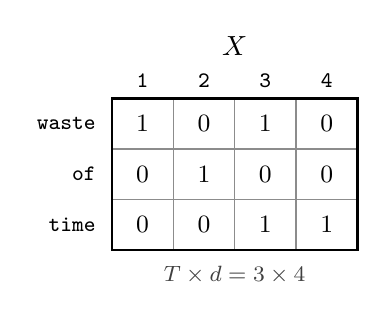
\begin{tikzpicture}
\draw[black!45, fill=white] (0.000,0.000) rectangle (0.780,-0.640);
\node[font=\small, text=black] at (0.390,-0.320) {$1$};
\draw[black!45, fill=white] (0.780,0.000) rectangle (1.560,-0.640);
\node[font=\small, text=black] at (1.170,-0.320) {$0$};
\draw[black!45, fill=white] (1.560,0.000) rectangle (2.340,-0.640);
\node[font=\small, text=black] at (1.950,-0.320) {$1$};
\draw[black!45, fill=white] (2.340,0.000) rectangle (3.120,-0.640);
\node[font=\small, text=black] at (2.730,-0.320) {$0$};
\draw[black!45, fill=white] (0.000,-0.640) rectangle (0.780,-1.279);
\node[font=\small, text=black] at (0.390,-0.959) {$0$};
\draw[black!45, fill=white] (0.780,-0.640) rectangle (1.560,-1.279);
\node[font=\small, text=black] at (1.170,-0.959) {$1$};
\draw[black!45, fill=white] (1.560,-0.640) rectangle (2.340,-1.279);
\node[font=\small, text=black] at (1.950,-0.959) {$0$};
\draw[black!45, fill=white] (2.340,-0.640) rectangle (3.120,-1.279);
\node[font=\small, text=black] at (2.730,-0.959) {$0$};
\draw[black!45, fill=white] (0.000,-1.279) rectangle (0.780,-1.919);
\node[font=\small, text=black] at (0.390,-1.599) {$0$};
\draw[black!45, fill=white] (0.780,-1.279) rectangle (1.560,-1.919);
\node[font=\small, text=black] at (1.170,-1.599) {$0$};
\draw[black!45, fill=white] (1.560,-1.279) rectangle (2.340,-1.919);
\node[font=\small, text=black] at (1.950,-1.599) {$1$};
\draw[black!45, fill=white] (2.340,-1.279) rectangle (3.120,-1.919);
\node[font=\small, text=black] at (2.730,-1.599) {$1$};
\draw[line width=0.9pt] (0.000,0.000) rectangle (3.120,-1.919);
\node[anchor=east, font=\footnotesize\ttfamily] at (-0.080,-0.320) {waste};
\node[anchor=east, font=\footnotesize\ttfamily] at (-0.080,-0.959) {of};
\node[anchor=east, font=\footnotesize\ttfamily] at (-0.080,-1.599) {time};
\node[anchor=south, font=\footnotesize\ttfamily] at (0.390,0.020) {1};
\node[anchor=south, font=\footnotesize\ttfamily] at (1.170,0.020) {2};
\node[anchor=south, font=\footnotesize\ttfamily] at (1.950,0.020) {3};
\node[anchor=south, font=\footnotesize\ttfamily] at (2.730,0.020) {4};
\node[anchor=south, font=\normalsize] at (1.560,0.420) {$X$};
\node[anchor=north, font=\footnotesize, text=black!75] at (1.560,-1.999) {$T\times d=3\times4$};
\end{tikzpicture}
\end{center}
These numbers are chosen by hand so you can follow every multiplication with a pencil. Real ones are learned
and much longer: Qwen3-0.6B uses 1024 numbers per token (Chapter 10).

%---------------------------------------------------------------------
\subsection*{3.1\quad The simple thing, and how it breaks}

Look at the token \tok{time}. On its own, its arrow is the same in every sentence: \emph{time flies}, \emph{on
time}, \emph{waste of time}. But the reply we want depends on \emph{wasted} time, time in a complaint. You learn
what kind of person someone is by talking to them, not by reading their name; a token learns what it means here
by listening to the tokens around it. So \tok{time} must pull in information from the tokens before it. What is
the simplest possible way? Take the average.

\Picture A class decides what to name the class pet, and every vote counts the same, whether the voter loves
the pet or has never seen it.

\Exactly
\[
\bm{u}_{\text{time}} = \tfrac{1}{3}\left(\bm{x}_{\text{waste}} + \bm{x}_{\text{of}} + \bm{x}_{\text{time}}\right) = \uTime \shape{1\times d}
\]
This says \tok{of} matters to \tok{time} exactly as much as \tok{waste} does. That is wrong, and no amount of
training can fix it, because there is nothing to train: the weights $\tfrac13,\tfrac13,\tfrac13$ are fixed by
the length of the sentence.

\begin{breaks}
In a class vote, every voter at least chose to vote. Here \tok{of} gets a full third of the say without having
anything to say about \tok{time}.
\end{breaks}

\Why \emph{We need the weights themselves to depend on the content}: \tok{time} should be able to \emph{ask}
which earlier tokens matter to it, and get a different answer in every sentence. To build ``asking'' and
``matching'' out of numbers, we need three tools from geometry. They are short, and they are the whole of the
mathematics in this chapter.

\begin{wrongidea}{3.1}
\emph{A token can use its own vector to predict the next word; mixing in other tokens is optional.} The vector
already encodes the word's meaning, so why mix? Because \tok{time}'s own vector is identical after \emph{on} and
after \emph{waste of}, and the right next word is different. Only the neighbours can tell them apart.
\end{wrongidea}

\begin{checkq}
Why can the token \tok{time} not predict \tok{Sorry} from its own arrow alone?
\begin{options}
\item It can: its arrow already encodes what \tok{time} means.
\item Its arrow is the same after \emph{on} and after \emph{waste of}, but the right next word differs.
\item It needs the plain average of all tokens, which settles the question.
\item Because its arrow does not know its position in the sentence.
\end{options}
\end{checkq}

\Summary{A token's own arrow is the same in every sentence, and a plain average cannot decide who matters, so
the mixing weights must depend on content.}

%---------------------------------------------------------------------
\subsection*{3.2\quad Tool 1: how much two arrows agree}

Start from something you may have built already: a churn score. For each customer you have some clues (days
since last login, support tickets this month, purchases this month) and for each clue an importance. The score
asks, for every clue, how important it is, and then combines everything together.

\Predict A customer has clues $\nThreeClues$ and the importances are $\nThreeW$. What is the score? Is it
positive or negative?

Multiply each clue by its importance and add: $\nThreeTerms = \nThreeScore$. Drawn as a row of clues
meeting a column of importances:
\begin{center}\resizebox{\linewidth}{!}{% AUTO-GENERATED by code/figlib.py helpers -- do not edit
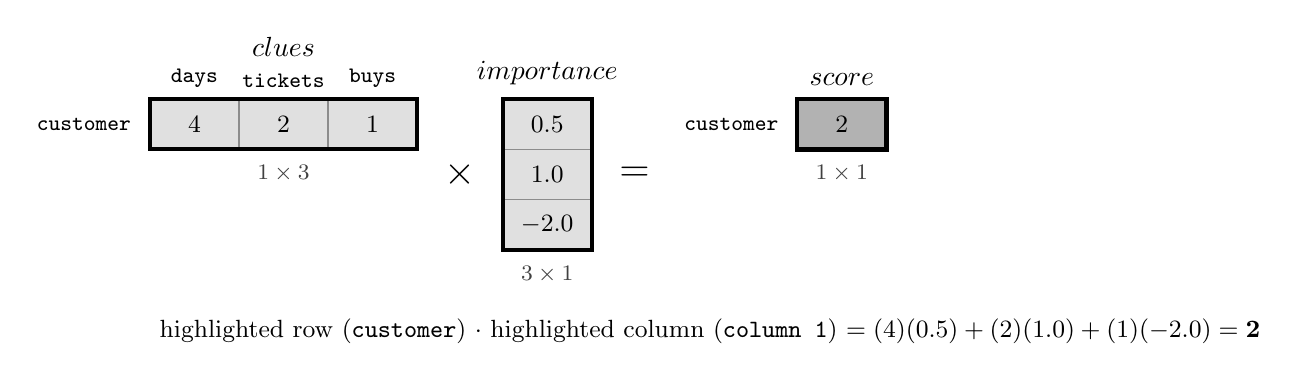
\begin{tikzpicture}[x=1.45cm]
\draw[black!45, fill=black!12] (0.000,0.000) rectangle (0.780,-0.640);
\node[font=\small, text=black] at (0.390,-0.320) {$4$};
\draw[black!45, fill=black!12] (0.780,0.000) rectangle (1.560,-0.640);
\node[font=\small, text=black] at (1.170,-0.320) {$2$};
\draw[black!45, fill=black!12] (1.560,0.000) rectangle (2.340,-0.640);
\node[font=\small, text=black] at (1.950,-0.320) {$1$};
\draw[line width=1.4pt] (0.000,0.000) rectangle (2.340,-0.640);
\draw[line width=0.9pt] (0.000,0.000) rectangle (2.340,-0.640);
\node[anchor=east, font=\footnotesize\ttfamily] at (-0.080,-0.320) {customer};
\node[anchor=south, font=\footnotesize\ttfamily] at (0.390,0.020) {days};
\node[anchor=south, font=\footnotesize\ttfamily] at (1.170,0.020) {tickets};
\node[anchor=south, font=\footnotesize\ttfamily] at (1.950,0.020) {buys};
\node[anchor=south, font=\normalsize] at (1.170,0.420) {$\text{clues}$};
\node[anchor=north, font=\footnotesize, text=black!75] at (1.170,-0.720) {$1\times3$};
\draw[black!45, fill=black!12] (3.090,0.000) rectangle (3.870,-0.640);
\node[font=\small, text=black] at (3.480,-0.320) {$0.5$};
\draw[black!45, fill=black!12] (3.090,-0.640) rectangle (3.870,-1.279);
\node[font=\small, text=black] at (3.480,-0.959) {$1.0$};
\draw[black!45, fill=black!12] (3.090,-1.279) rectangle (3.870,-1.919);
\node[font=\small, text=black] at (3.480,-1.599) {$-2.0$};
\draw[line width=1.4pt] (3.090,0.000) rectangle (3.870,-1.919);
\draw[line width=0.9pt] (3.090,0.000) rectangle (3.870,-1.919);
\node[anchor=south, font=\normalsize] at (3.480,0.050) {$\text{importance}$};
\node[anchor=north, font=\footnotesize, text=black!75] at (3.480,-1.999) {$3\times1$};
\draw[black!45, fill=black!30] (5.670,0.000) rectangle (6.450,-0.640);
\node[font=\small, text=black] at (6.060,-0.320) {$2$};
\draw[line width=1.6pt] (5.670,0.000) rectangle (6.450,-0.640);
\draw[line width=0.9pt] (5.670,0.000) rectangle (6.450,-0.640);
\node[anchor=east, font=\footnotesize\ttfamily] at (5.590,-0.320) {customer};
\node[anchor=south, font=\normalsize] at (6.060,0.050) {$\text{score}$};
\node[anchor=north, font=\footnotesize, text=black!75] at (6.060,-0.720) {$1\times1$};
\node[font=\Large] at (2.715,-0.959) {$\times$};
\node[font=\Large] at (4.245,-0.959) {$=$};
\node[anchor=north west, font=\small, align=left] at (0,-2.669) {highlighted row (\texttt{customer}) $\cdot$ highlighted column (\texttt{column 1}) $= (4)(0.5) + (2)(1.0) + (1)(-2.0) = \mathbf{2}$};
\end{tikzpicture}
}\end{center}

That operation, multiply matching entries and add, is the \emph{dot product}. Now let us see it as geometry.

\Picture An arrow is a set of directions: ``3 steps east, 1 step north'' is the arrow $(3,1)$. Two friends walk
out of school, one along $\bm{a}=(3,1)$ and one along $\bm{b}=(1,2)$. How much are they going \emph{the same
way}? Shine a torch from straight above $\bm{a}$'s path and look at the shadow that $\bm{b}$ casts on it. A long
shadow means they mostly agree. No shadow means they are walking at right angles. A shadow pointing backwards
means they are walking apart.

\begin{figure}[h]
\centering
\begin{tikzpicture}[scale=1.05, font=\footnotesize]
\draw[black!50] (-0.3,0) -- (3.6,0); \draw[black!50] (0,-0.3) -- (0,1.8);
\draw[-{Stealth}, thick] (0,0) -- (3,1) node[right] {$\bm{a}=(3,1)$, length \geoNa};
\draw[-{Stealth}, thick, black!70] (0,0) -- (1,2) node[above, text=black] {$\bm{b}=(1,2)$, length \geoNb};
\draw[dashed] (1,2) -- (1.5,0.5);
\draw[line width=2.4pt, black!35] (0,0) -- (1.5,0.5);
\node[below right, align=left] at (1.35,0.35) {shadow of $\bm{b}$ on $\bm{a}$:\\length \geoShadow};
\draw (0.55,0.183) arc[start angle=18.43, end angle=63.43, radius=0.58];
\node at (0.62,0.62) {\geoAng$^\circ$};
\begin{scope}[xshift=7.2cm, scale=0.55]
\foreach \y/\lab/\bx/\by in {3.2/{same way: big, positive}/2/0.6, 0/{right angle: zero}/0/1.6, -3.2/{opposite: negative}/-1.5/0.9} {
  \draw[-{Stealth}, thick] (0,\y) -- (2,\y+0.6);
  \draw[-{Stealth}, thick, black!60] (0,\y) -- (\bx,\y+\by);
  \node[right, font=\footnotesize] at (2.6,\y+0.3) {\lab};
}
\end{scope}
\end{tikzpicture}
\caption{The dot product as a shadow. Left: our two arrows, at \geoAng$^\circ$. Right: the three cases.}
\label{fig:dot}
\end{figure}

\Predict Before computing $(3,1)\cdot(1,2)$: from the picture, will it be positive, zero or negative?

\Exactly The dot product multiplies matching entries and adds:
\[
\bm{a}\cdot\bm{b} = a_1b_1 + a_2b_2 + \cdots + a_db_d .
\]
As a picture, the row $\bm{a}$ meets the column $\bm{b}$ (we write $\bm{b}$ standing up, as $\bm{b}^\top$):
\begin{center}% AUTO-GENERATED by code/figlib.py helpers -- do not edit
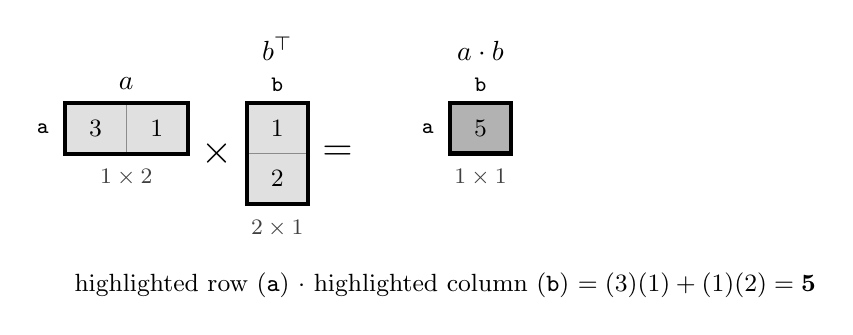
\begin{tikzpicture}
\draw[black!45, fill=black!12] (0.000,0.000) rectangle (0.780,-0.640);
\node[font=\small, text=black] at (0.390,-0.320) {$3$};
\draw[black!45, fill=black!12] (0.780,0.000) rectangle (1.560,-0.640);
\node[font=\small, text=black] at (1.170,-0.320) {$1$};
\draw[line width=1.4pt] (0.000,0.000) rectangle (1.560,-0.640);
\draw[line width=0.9pt] (0.000,0.000) rectangle (1.560,-0.640);
\node[anchor=east, font=\footnotesize\ttfamily] at (-0.080,-0.320) {a};
\node[anchor=south, font=\normalsize] at (0.780,0.050) {$\bm{a}$};
\node[anchor=north, font=\footnotesize, text=black!75] at (0.780,-0.720) {$1\times2$};
\draw[black!45, fill=black!12] (2.310,0.000) rectangle (3.090,-0.640);
\node[font=\small, text=black] at (2.700,-0.320) {$1$};
\draw[black!45, fill=black!12] (2.310,-0.640) rectangle (3.090,-1.279);
\node[font=\small, text=black] at (2.700,-0.959) {$2$};
\draw[line width=1.4pt] (2.310,0.000) rectangle (3.090,-1.279);
\draw[line width=0.9pt] (2.310,0.000) rectangle (3.090,-1.279);
\node[anchor=south, font=\footnotesize\ttfamily] at (2.700,0.020) {b};
\node[anchor=south, font=\normalsize] at (2.700,0.420) {$\bm{b}^{\top}$};
\node[anchor=north, font=\footnotesize, text=black!75] at (2.700,-1.359) {$2\times1$};
\draw[black!45, fill=black!30] (4.890,0.000) rectangle (5.670,-0.640);
\node[font=\small, text=black] at (5.280,-0.320) {$5$};
\draw[line width=1.6pt] (4.890,0.000) rectangle (5.670,-0.640);
\draw[line width=0.9pt] (4.890,0.000) rectangle (5.670,-0.640);
\node[anchor=east, font=\footnotesize\ttfamily] at (4.810,-0.320) {a};
\node[anchor=south, font=\footnotesize\ttfamily] at (5.280,0.020) {b};
\node[anchor=south, font=\normalsize] at (5.280,0.420) {$\bm{a}\cdot\bm{b}$};
\node[anchor=north, font=\footnotesize, text=black!75] at (5.280,-0.720) {$1\times1$};
\node[font=\Large] at (1.935,-0.640) {$\times$};
\node[font=\Large] at (3.465,-0.640) {$=$};
\node[anchor=north west, font=\small, align=left] at (0,-2.029) {highlighted row (\texttt{a}) $\cdot$ highlighted column (\texttt{b}) $= (3)(1) + (1)(2) = \mathbf{5}$};
\end{tikzpicture}
\end{center}
The surprising fact is that this sum measures agreement:
\[
\bm{a}\cdot\bm{b} \;=\; \lVert\bm{a}\rVert\,\lVert\bm{b}\rVert\cos\theta ,
\]
where $\theta$ is the angle between the arrows. Check it: $\geoNa \times \geoNb \times \cos \geoAng^\circ =
\geoDot$. Why should multiply-and-add know about angles? Draw the third side of the triangle, $\bm{a}-\bm{b}$.
Expanding its squared length entry by entry gives $\lVert\bm{a}-\bm{b}\rVert^2 = \lVert\bm{a}\rVert^2 +
\lVert\bm{b}\rVert^2 - 2\,\bm{a}\cdot\bm{b}$, while the law of cosines says the same squared length is
$\lVert\bm{a}\rVert^2 + \lVert\bm{b}\rVert^2 - 2\lVert\bm{a}\rVert\lVert\bm{b}\rVert\cos\theta$. Compare the two,
and the formula falls out. Nothing in the argument cares whether there are 2 entries or 1024, so the picture
holds in any number of dimensions.

\Sanity The churn customer is an arrow too: three clues, three directions. Its score of \nThreeScore\ is the
shadow of the customer arrow on the importance arrow, times the importance arrow's length.

\begin{breaks}
You can draw shadows in two or three dimensions. In 1024 dimensions you cannot, but the arithmetic still works
and still means ``how much do these agree''. Trust the formula where the drawing stops.
\end{breaks}

\Why The dot product has exactly two knobs: \emph{direction} ($\cos\theta$, how much the arrows agree) and
\emph{length} ($\lVert\bm{a}\rVert\lVert\bm{b}\rVert$, how strongly they say it). Keep these two knobs in mind; at
the end of the chapter, learning will turn out to be nothing but turning them.

\begin{wrongidea}{3.8}
\emph{A bigger dot product always means more similar.} Dot products are often introduced as similarity scores,
so bigger feels like closer. But a long arrow pointing a little off can beat a short arrow pointing exactly the
same way. Similarity of direction is $\cos\theta$; the dot product also multiplies in both lengths.
\end{wrongidea}

\begin{checkq}
Take $\bm{a}=(1,0)$, $\bm{b}=(3,3)$ and $\bm{c}=(1,0)$. Which arrow points most nearly the same way as $\bm{a}$?
\begin{options}
\item $\bm{b}$, because $\bm{a}\cdot\bm{b}=\nThreeQbDot$ is bigger than $\bm{a}\cdot\bm{c}=\nThreeQcDot$.
\item $\bm{c}$: the angle is \nThreeQcAng$^\circ$, against \nThreeQbAng$^\circ$ for $\bm{b}$.
\item They agree equally, since both dot products are positive.
\item You cannot tell without drawing them.
\end{options}
\end{checkq}

\Summary{Multiply-and-add measures how much two arrows agree in direction, scaled by how long they are.}

%---------------------------------------------------------------------
\subsection*{3.3\quad Tool 2: a matrix is a machine that moves arrows}

\Picture A matrix is a set of recipe cards. Each card says ``take this much of your first number, this much of
your second, \ldots, and add''. An arrow goes in; each card produces one number of the new arrow. A matrix with
64 columns is 64 recipes: 64 different ways of looking at the same token.

\Exactly Multiplying a $1\times d$ arrow by a $d\times d_k$ matrix $W$ gives a $1\times d_k$ arrow whose $j$-th
entry is the dot product of the input with column $j$ of $W$ (card $j$).

\Predict Feed \tok{waste}, $(1,0,1,0)$, into the key matrix below. Before multiplying: which rows of $W_K$ will
end up mattering?
\begin{center}% AUTO-GENERATED by code/figlib.py helpers -- do not edit
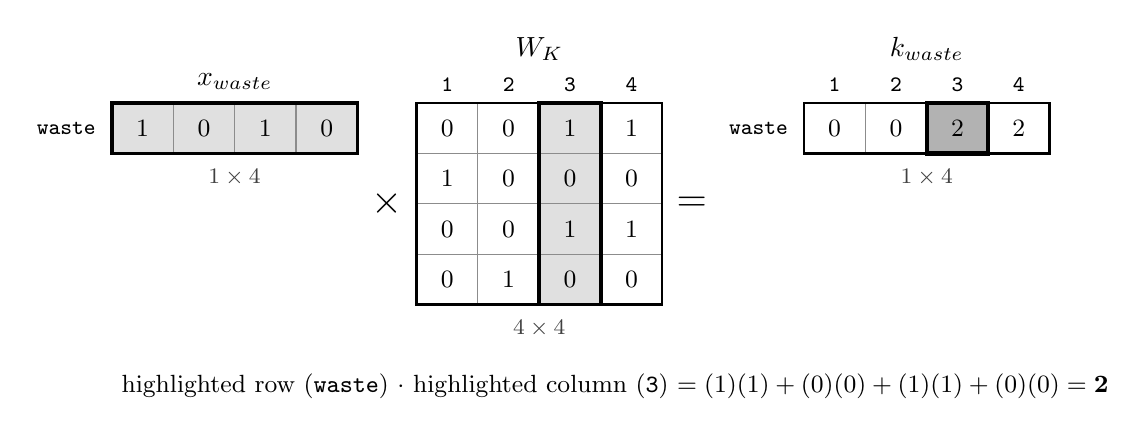
\begin{tikzpicture}
\draw[black!45, fill=black!12] (0.000,0.000) rectangle (0.780,-0.640);
\node[font=\small, text=black] at (0.390,-0.320) {$1$};
\draw[black!45, fill=black!12] (0.780,0.000) rectangle (1.560,-0.640);
\node[font=\small, text=black] at (1.170,-0.320) {$0$};
\draw[black!45, fill=black!12] (1.560,0.000) rectangle (2.340,-0.640);
\node[font=\small, text=black] at (1.950,-0.320) {$1$};
\draw[black!45, fill=black!12] (2.340,0.000) rectangle (3.120,-0.640);
\node[font=\small, text=black] at (2.730,-0.320) {$0$};
\draw[line width=1.4pt] (0.000,0.000) rectangle (3.120,-0.640);
\draw[line width=0.9pt] (0.000,0.000) rectangle (3.120,-0.640);
\node[anchor=east, font=\footnotesize\ttfamily] at (-0.080,-0.320) {waste};
\node[anchor=south, font=\normalsize] at (1.560,0.050) {$\bm{x}_{\text{waste}}$};
\node[anchor=north, font=\footnotesize, text=black!75] at (1.560,-0.720) {$1\times4$};
\draw[black!45, fill=white] (3.870,0.000) rectangle (4.650,-0.640);
\node[font=\small, text=black] at (4.260,-0.320) {$0$};
\draw[black!45, fill=white] (4.650,0.000) rectangle (5.430,-0.640);
\node[font=\small, text=black] at (5.040,-0.320) {$0$};
\draw[black!45, fill=black!12] (5.430,0.000) rectangle (6.210,-0.640);
\node[font=\small, text=black] at (5.820,-0.320) {$1$};
\draw[black!45, fill=white] (6.210,0.000) rectangle (6.990,-0.640);
\node[font=\small, text=black] at (6.600,-0.320) {$1$};
\draw[black!45, fill=white] (3.870,-0.640) rectangle (4.650,-1.279);
\node[font=\small, text=black] at (4.260,-0.959) {$1$};
\draw[black!45, fill=white] (4.650,-0.640) rectangle (5.430,-1.279);
\node[font=\small, text=black] at (5.040,-0.959) {$0$};
\draw[black!45, fill=black!12] (5.430,-0.640) rectangle (6.210,-1.279);
\node[font=\small, text=black] at (5.820,-0.959) {$0$};
\draw[black!45, fill=white] (6.210,-0.640) rectangle (6.990,-1.279);
\node[font=\small, text=black] at (6.600,-0.959) {$0$};
\draw[black!45, fill=white] (3.870,-1.279) rectangle (4.650,-1.919);
\node[font=\small, text=black] at (4.260,-1.599) {$0$};
\draw[black!45, fill=white] (4.650,-1.279) rectangle (5.430,-1.919);
\node[font=\small, text=black] at (5.040,-1.599) {$0$};
\draw[black!45, fill=black!12] (5.430,-1.279) rectangle (6.210,-1.919);
\node[font=\small, text=black] at (5.820,-1.599) {$1$};
\draw[black!45, fill=white] (6.210,-1.279) rectangle (6.990,-1.919);
\node[font=\small, text=black] at (6.600,-1.599) {$1$};
\draw[black!45, fill=white] (3.870,-1.919) rectangle (4.650,-2.558);
\node[font=\small, text=black] at (4.260,-2.239) {$0$};
\draw[black!45, fill=white] (4.650,-1.919) rectangle (5.430,-2.558);
\node[font=\small, text=black] at (5.040,-2.239) {$1$};
\draw[black!45, fill=black!12] (5.430,-1.919) rectangle (6.210,-2.558);
\node[font=\small, text=black] at (5.820,-2.239) {$0$};
\draw[black!45, fill=white] (6.210,-1.919) rectangle (6.990,-2.558);
\node[font=\small, text=black] at (6.600,-2.239) {$0$};
\draw[line width=1.4pt] (5.430,0.000) rectangle (6.210,-2.558);
\draw[line width=0.9pt] (3.870,0.000) rectangle (6.990,-2.558);
\node[anchor=south, font=\footnotesize\ttfamily] at (4.260,0.020) {1};
\node[anchor=south, font=\footnotesize\ttfamily] at (5.040,0.020) {2};
\node[anchor=south, font=\footnotesize\ttfamily] at (5.820,0.020) {3};
\node[anchor=south, font=\footnotesize\ttfamily] at (6.600,0.020) {4};
\node[anchor=south, font=\normalsize] at (5.430,0.420) {$W_K$};
\node[anchor=north, font=\footnotesize, text=black!75] at (5.430,-2.638) {$4\times4$};
\draw[black!45, fill=white] (8.790,0.000) rectangle (9.570,-0.640);
\node[font=\small, text=black] at (9.180,-0.320) {$0$};
\draw[black!45, fill=white] (9.570,0.000) rectangle (10.350,-0.640);
\node[font=\small, text=black] at (9.960,-0.320) {$0$};
\draw[black!45, fill=black!30] (10.350,0.000) rectangle (11.130,-0.640);
\node[font=\small, text=black] at (10.740,-0.320) {$2$};
\draw[black!45, fill=white] (11.130,0.000) rectangle (11.910,-0.640);
\node[font=\small, text=black] at (11.520,-0.320) {$2$};
\draw[line width=1.6pt] (10.350,0.000) rectangle (11.130,-0.640);
\draw[line width=0.9pt] (8.790,0.000) rectangle (11.910,-0.640);
\node[anchor=east, font=\footnotesize\ttfamily] at (8.710,-0.320) {waste};
\node[anchor=south, font=\footnotesize\ttfamily] at (9.180,0.020) {1};
\node[anchor=south, font=\footnotesize\ttfamily] at (9.960,0.020) {2};
\node[anchor=south, font=\footnotesize\ttfamily] at (10.740,0.020) {3};
\node[anchor=south, font=\footnotesize\ttfamily] at (11.520,0.020) {4};
\node[anchor=south, font=\normalsize] at (10.350,0.420) {$\bm{k}_{\text{waste}}$};
\node[anchor=north, font=\footnotesize, text=black!75] at (10.350,-0.720) {$1\times4$};
\node[font=\Large] at (3.495,-1.279) {$\times$};
\node[font=\Large] at (7.365,-1.279) {$=$};
\node[anchor=north west, font=\small, align=left] at (0,-3.308) {highlighted row (\texttt{waste}) $\cdot$ highlighted column (\texttt{3}) $= (1)(1) + (0)(0) + (1)(1) + (0)(0) = \mathbf{2}$};
\end{tikzpicture}
\end{center}
Each output number is the input row meeting one column (one recipe card). The highlighted column 3 gives 2; the
four columns give $\kWasteRow$. There is a second way to see the same multiplication. Because $\bm{x}_{\text{waste}}$ has a 1 in positions 1 and 3,
the result is \emph{row 1 plus row 3} of $W_K$, namely $(0,0,1,1)+(0,0,1,1)$. A matrix sends each input direction
somewhere; it can rotate arrows, stretch them, squash them, or flatten some directions to nothing.

\begin{breaks}
Recipe cards suggest each card is separate. A matrix also has a single geometric effect on the whole space (a
turn, a stretch, a squash) that no single card shows.
\end{breaks}

\Why A matrix lets the \emph{same} token be seen in different ways. The arrow for \tok{waste} is fixed, but $W_K$
produces one view of it and $W_Q$ another. If the model needs a new view, it does not change the word; it learns
a new machine.

\Summary{A matrix turns one arrow into another, one recipe (column) per output number, so one token can be viewed
in many learned ways.}

%---------------------------------------------------------------------
\subsection*{3.4\quad Tool 3: the transpose, and the table of all meetings}

\Picture At the start of a tournament every player shakes hands with every other player. The organiser draws a
table: players down the side, players across the top, and in each cell writes how friendly that handshake was.

\Exactly Stack all the queries as rows of $Q$ ($T\times d_k$) and all the keys as rows of $K$ ($T\times d_k$). We
want the table $S$ with $S_{ij} = \bm{q}_i\cdot\bm{k}_j$. Matrix multiplication always pairs a \emph{row of the
left} with a \emph{column of the right}. Our queries are already rows. Our keys are rows too, so we flip them into
columns: that flip is the \emph{transpose} $K^\top$ ($d_k\times T$). Now
\[
S = Q K^\top \shape{(T\times d_k)(d_k\times T) = T\times T},
\]
and the cell in row $i$, column $j$ is row $i$ of $Q$ meeting column $j$ of $K^\top$, which is
$\bm{q}_i\cdot\bm{k}_j$. There is a deeper way to see it. A column of $K^\top$ is a key, and dot-producting with
an arrow measures the shadow along it. So $K^\top$ is a set of $T$ \emph{rulers}, one per key, and multiplying a
query by $K^\top$ measures that query along every key at once.

\begin{breaks}
A handshake is the same from both sides. Here it is not: the score of \tok{time} looking at \tok{waste} uses
\tok{time}'s query and \tok{waste}'s key, while \tok{waste} looking at \tok{time} uses the other pair. The table is
not symmetric.
\end{breaks}

\Why This is Requirement 4 in one line. An RNN produces its numbers one step after another; here all $T\times T$
scores come out of a single matrix multiplication, which is the operation a GPU's thousands of workers are built
to share.

\begin{wrongidea}{3.9}
\emph{The transpose changes the vectors.} The matrix looks different afterwards, so something must have changed.
But every key arrow is exactly the same arrow before and after; the transpose only stands it up as a column, so
that ``row meets column'' pairs each query with each key.
\end{wrongidea}

\begin{checkq}
In $QK^\top$ for our toy, why $K^\top$ and not $K$?
\begin{options}
\item $Q$ is $3\times4$ and $K$ is $3\times4$, so $QK$ is not defined; $QK^\top$ is $3\times3$, one score per pair of tokens.
\item The transpose turns the keys so they match the queries better.
\item The transpose rescales the keys to length 1.
\item Either works; $QK$ gives the same numbers in a different order.
\end{options}
\end{checkq}

\Summary{Flipping the keys into columns lets one multiplication produce every query-key score at once, without
changing any arrow.}

%---------------------------------------------------------------------
\subsection*{3.5\quad The fix: three questions per token}

Now we can build ``asking''. Attention gives every token three different views of itself, each made by its own
learned machine:
\begin{itemize}
\item \textbf{Query} $\bm{q}=\bm{x}W_Q$: \emph{what am I looking for?}
\item \textbf{Key} $\bm{k}=\bm{x}W_K$: \emph{what can I be found by?}
\item \textbf{Value} $\bm{v}=\bm{x}W_V$: \emph{what do I hand over if I am chosen?}
\end{itemize}

\Picture A library. The query is what you type into the search box. The key is the label on each book's spine.
The value is what is written inside the book. You match your search against the labels, but you take home the
contents.

\begin{breaks}
In a library you take home a few whole books. Attention takes home a blend: a little of every book, in
proportions set by how well each label matched.
\end{breaks}

\Why Why three, and not one arrow for everything? Because what makes you \emph{findable} is not the same as what
you \emph{offer}, and neither is the same as what you \emph{need}. \tok{waste} should be found by any token asking
``is there a judgement nearby?'', but what it hands over is the content of that judgement, and what \tok{waste}
itself is looking for is something else again. One arrow cannot point in three directions.

\begin{wrongidea}{3.4}
\emph{Query, key and value are three copies of the same thing; one vector would do.} All three are made from the
same token arrow, so they look like copies. The paragraph above explains why they are not: each is a different
machine applied to the same arrow, and each points where its own job needs it.
\end{wrongidea}

\begin{wrongidea}{3.6}
\emph{Values are the words' original meanings.} Values are made from the embeddings, so it is tempting to read
them as the dictionary meaning. They are a learned \emph{view} made for handing over, built by $W_V$. In the toy,
$\bm{x}_{\text{waste}}=(1,0,1,0)$ but $\bm{v}_{\text{waste}}$ is different, as you will see below.
\end{wrongidea}

In the toy we use the machines in Figure~\ref{fig:qkv} (chosen for pencil-friendliness; real ones are
learned). Each picture feeds all three tokens through one machine at once: $X$ ($3\times4$) times $W$ ($4\times4$)
gives one new row per token. One row meeting one column is highlighted and written out; check one more cell
yourself before reading on.
\begin{figure}[!htb]\centering
% AUTO-GENERATED by code/figlib.py helpers -- do not edit
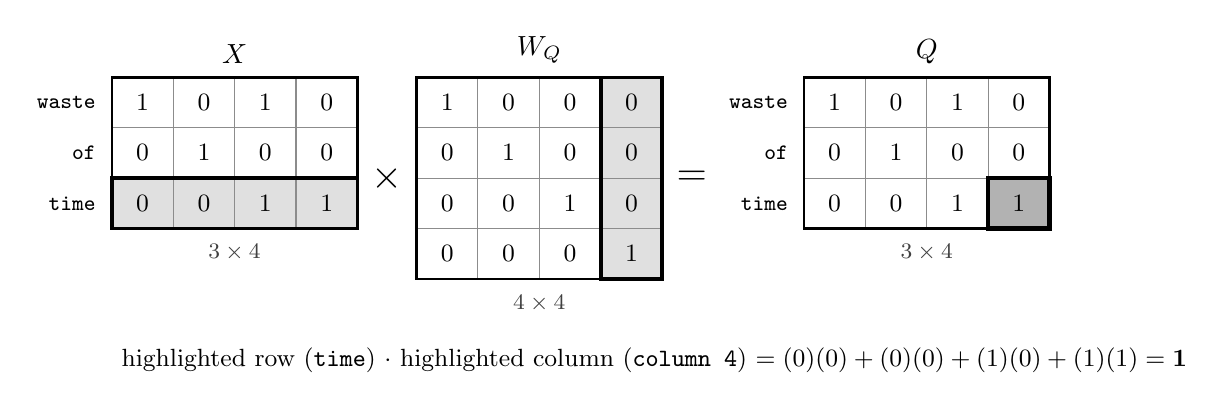
\begin{tikzpicture}
\draw[black!45, fill=white] (0.000,0.000) rectangle (0.780,-0.640);
\node[font=\small, text=black] at (0.390,-0.320) {$1$};
\draw[black!45, fill=white] (0.780,0.000) rectangle (1.560,-0.640);
\node[font=\small, text=black] at (1.170,-0.320) {$0$};
\draw[black!45, fill=white] (1.560,0.000) rectangle (2.340,-0.640);
\node[font=\small, text=black] at (1.950,-0.320) {$1$};
\draw[black!45, fill=white] (2.340,0.000) rectangle (3.120,-0.640);
\node[font=\small, text=black] at (2.730,-0.320) {$0$};
\draw[black!45, fill=white] (0.000,-0.640) rectangle (0.780,-1.279);
\node[font=\small, text=black] at (0.390,-0.959) {$0$};
\draw[black!45, fill=white] (0.780,-0.640) rectangle (1.560,-1.279);
\node[font=\small, text=black] at (1.170,-0.959) {$1$};
\draw[black!45, fill=white] (1.560,-0.640) rectangle (2.340,-1.279);
\node[font=\small, text=black] at (1.950,-0.959) {$0$};
\draw[black!45, fill=white] (2.340,-0.640) rectangle (3.120,-1.279);
\node[font=\small, text=black] at (2.730,-0.959) {$0$};
\draw[black!45, fill=black!12] (0.000,-1.279) rectangle (0.780,-1.919);
\node[font=\small, text=black] at (0.390,-1.599) {$0$};
\draw[black!45, fill=black!12] (0.780,-1.279) rectangle (1.560,-1.919);
\node[font=\small, text=black] at (1.170,-1.599) {$0$};
\draw[black!45, fill=black!12] (1.560,-1.279) rectangle (2.340,-1.919);
\node[font=\small, text=black] at (1.950,-1.599) {$1$};
\draw[black!45, fill=black!12] (2.340,-1.279) rectangle (3.120,-1.919);
\node[font=\small, text=black] at (2.730,-1.599) {$1$};
\draw[line width=1.4pt] (0.000,-1.279) rectangle (3.120,-1.919);
\draw[line width=0.9pt] (0.000,0.000) rectangle (3.120,-1.919);
\node[anchor=east, font=\footnotesize\ttfamily] at (-0.080,-0.320) {waste};
\node[anchor=east, font=\footnotesize\ttfamily] at (-0.080,-0.959) {of};
\node[anchor=east, font=\footnotesize\ttfamily] at (-0.080,-1.599) {time};
\node[anchor=south, font=\normalsize] at (1.560,0.050) {$X$};
\node[anchor=north, font=\footnotesize, text=black!75] at (1.560,-1.999) {$3\times4$};
\draw[black!45, fill=white] (3.870,0.000) rectangle (4.650,-0.640);
\node[font=\small, text=black] at (4.260,-0.320) {$1$};
\draw[black!45, fill=white] (4.650,0.000) rectangle (5.430,-0.640);
\node[font=\small, text=black] at (5.040,-0.320) {$0$};
\draw[black!45, fill=white] (5.430,0.000) rectangle (6.210,-0.640);
\node[font=\small, text=black] at (5.820,-0.320) {$0$};
\draw[black!45, fill=black!12] (6.210,0.000) rectangle (6.990,-0.640);
\node[font=\small, text=black] at (6.600,-0.320) {$0$};
\draw[black!45, fill=white] (3.870,-0.640) rectangle (4.650,-1.279);
\node[font=\small, text=black] at (4.260,-0.959) {$0$};
\draw[black!45, fill=white] (4.650,-0.640) rectangle (5.430,-1.279);
\node[font=\small, text=black] at (5.040,-0.959) {$1$};
\draw[black!45, fill=white] (5.430,-0.640) rectangle (6.210,-1.279);
\node[font=\small, text=black] at (5.820,-0.959) {$0$};
\draw[black!45, fill=black!12] (6.210,-0.640) rectangle (6.990,-1.279);
\node[font=\small, text=black] at (6.600,-0.959) {$0$};
\draw[black!45, fill=white] (3.870,-1.279) rectangle (4.650,-1.919);
\node[font=\small, text=black] at (4.260,-1.599) {$0$};
\draw[black!45, fill=white] (4.650,-1.279) rectangle (5.430,-1.919);
\node[font=\small, text=black] at (5.040,-1.599) {$0$};
\draw[black!45, fill=white] (5.430,-1.279) rectangle (6.210,-1.919);
\node[font=\small, text=black] at (5.820,-1.599) {$1$};
\draw[black!45, fill=black!12] (6.210,-1.279) rectangle (6.990,-1.919);
\node[font=\small, text=black] at (6.600,-1.599) {$0$};
\draw[black!45, fill=white] (3.870,-1.919) rectangle (4.650,-2.558);
\node[font=\small, text=black] at (4.260,-2.239) {$0$};
\draw[black!45, fill=white] (4.650,-1.919) rectangle (5.430,-2.558);
\node[font=\small, text=black] at (5.040,-2.239) {$0$};
\draw[black!45, fill=white] (5.430,-1.919) rectangle (6.210,-2.558);
\node[font=\small, text=black] at (5.820,-2.239) {$0$};
\draw[black!45, fill=black!12] (6.210,-1.919) rectangle (6.990,-2.558);
\node[font=\small, text=black] at (6.600,-2.239) {$1$};
\draw[line width=1.4pt] (6.210,0.000) rectangle (6.990,-2.558);
\draw[line width=0.9pt] (3.870,0.000) rectangle (6.990,-2.558);
\node[anchor=south, font=\normalsize] at (5.430,0.050) {$W_Q$};
\node[anchor=north, font=\footnotesize, text=black!75] at (5.430,-2.638) {$4\times4$};
\draw[black!45, fill=white] (8.790,0.000) rectangle (9.570,-0.640);
\node[font=\small, text=black] at (9.180,-0.320) {$1$};
\draw[black!45, fill=white] (9.570,0.000) rectangle (10.350,-0.640);
\node[font=\small, text=black] at (9.960,-0.320) {$0$};
\draw[black!45, fill=white] (10.350,0.000) rectangle (11.130,-0.640);
\node[font=\small, text=black] at (10.740,-0.320) {$1$};
\draw[black!45, fill=white] (11.130,0.000) rectangle (11.910,-0.640);
\node[font=\small, text=black] at (11.520,-0.320) {$0$};
\draw[black!45, fill=white] (8.790,-0.640) rectangle (9.570,-1.279);
\node[font=\small, text=black] at (9.180,-0.959) {$0$};
\draw[black!45, fill=white] (9.570,-0.640) rectangle (10.350,-1.279);
\node[font=\small, text=black] at (9.960,-0.959) {$1$};
\draw[black!45, fill=white] (10.350,-0.640) rectangle (11.130,-1.279);
\node[font=\small, text=black] at (10.740,-0.959) {$0$};
\draw[black!45, fill=white] (11.130,-0.640) rectangle (11.910,-1.279);
\node[font=\small, text=black] at (11.520,-0.959) {$0$};
\draw[black!45, fill=white] (8.790,-1.279) rectangle (9.570,-1.919);
\node[font=\small, text=black] at (9.180,-1.599) {$0$};
\draw[black!45, fill=white] (9.570,-1.279) rectangle (10.350,-1.919);
\node[font=\small, text=black] at (9.960,-1.599) {$0$};
\draw[black!45, fill=white] (10.350,-1.279) rectangle (11.130,-1.919);
\node[font=\small, text=black] at (10.740,-1.599) {$1$};
\draw[black!45, fill=black!30] (11.130,-1.279) rectangle (11.910,-1.919);
\node[font=\small, text=black] at (11.520,-1.599) {$1$};
\draw[line width=1.6pt] (11.130,-1.279) rectangle (11.910,-1.919);
\draw[line width=0.9pt] (8.790,0.000) rectangle (11.910,-1.919);
\node[anchor=east, font=\footnotesize\ttfamily] at (8.710,-0.320) {waste};
\node[anchor=east, font=\footnotesize\ttfamily] at (8.710,-0.959) {of};
\node[anchor=east, font=\footnotesize\ttfamily] at (8.710,-1.599) {time};
\node[anchor=south, font=\normalsize] at (10.350,0.050) {$Q$};
\node[anchor=north, font=\footnotesize, text=black!75] at (10.350,-1.999) {$3\times4$};
\node[font=\Large] at (3.495,-1.279) {$\times$};
\node[font=\Large] at (7.365,-1.279) {$=$};
\node[anchor=north west, font=\small, align=left] at (0,-3.308) {highlighted row (\texttt{time}) $\cdot$ highlighted column (\texttt{column 4}) $= (0)(0) + (0)(0) + (1)(0) + (1)(1) = \mathbf{1}$};
\end{tikzpicture}
\\[10pt]
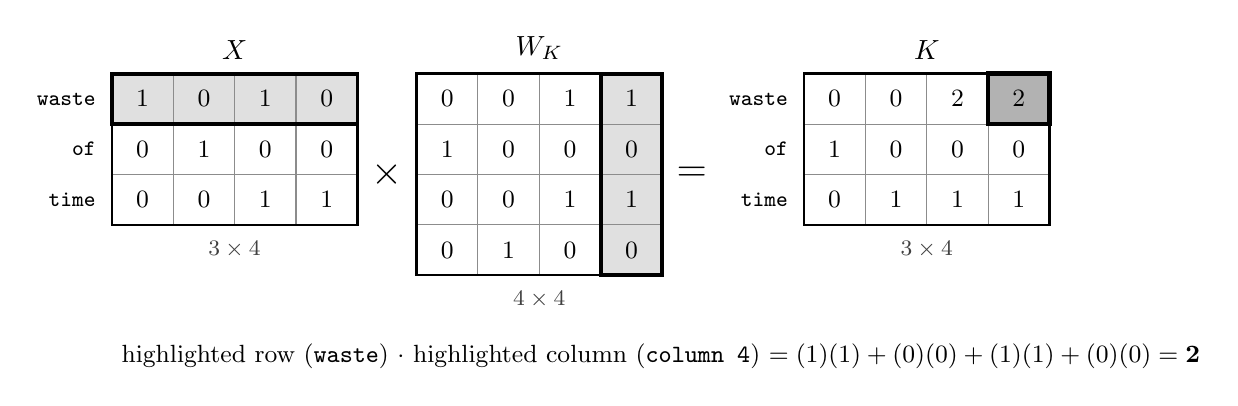
\begin{tikzpicture}
\draw[black!45, fill=black!12] (0.000,0.000) rectangle (0.780,-0.640);
\node[font=\small, text=black] at (0.390,-0.320) {$1$};
\draw[black!45, fill=black!12] (0.780,0.000) rectangle (1.560,-0.640);
\node[font=\small, text=black] at (1.170,-0.320) {$0$};
\draw[black!45, fill=black!12] (1.560,0.000) rectangle (2.340,-0.640);
\node[font=\small, text=black] at (1.950,-0.320) {$1$};
\draw[black!45, fill=black!12] (2.340,0.000) rectangle (3.120,-0.640);
\node[font=\small, text=black] at (2.730,-0.320) {$0$};
\draw[black!45, fill=white] (0.000,-0.640) rectangle (0.780,-1.279);
\node[font=\small, text=black] at (0.390,-0.959) {$0$};
\draw[black!45, fill=white] (0.780,-0.640) rectangle (1.560,-1.279);
\node[font=\small, text=black] at (1.170,-0.959) {$1$};
\draw[black!45, fill=white] (1.560,-0.640) rectangle (2.340,-1.279);
\node[font=\small, text=black] at (1.950,-0.959) {$0$};
\draw[black!45, fill=white] (2.340,-0.640) rectangle (3.120,-1.279);
\node[font=\small, text=black] at (2.730,-0.959) {$0$};
\draw[black!45, fill=white] (0.000,-1.279) rectangle (0.780,-1.919);
\node[font=\small, text=black] at (0.390,-1.599) {$0$};
\draw[black!45, fill=white] (0.780,-1.279) rectangle (1.560,-1.919);
\node[font=\small, text=black] at (1.170,-1.599) {$0$};
\draw[black!45, fill=white] (1.560,-1.279) rectangle (2.340,-1.919);
\node[font=\small, text=black] at (1.950,-1.599) {$1$};
\draw[black!45, fill=white] (2.340,-1.279) rectangle (3.120,-1.919);
\node[font=\small, text=black] at (2.730,-1.599) {$1$};
\draw[line width=1.4pt] (0.000,0.000) rectangle (3.120,-0.640);
\draw[line width=0.9pt] (0.000,0.000) rectangle (3.120,-1.919);
\node[anchor=east, font=\footnotesize\ttfamily] at (-0.080,-0.320) {waste};
\node[anchor=east, font=\footnotesize\ttfamily] at (-0.080,-0.959) {of};
\node[anchor=east, font=\footnotesize\ttfamily] at (-0.080,-1.599) {time};
\node[anchor=south, font=\normalsize] at (1.560,0.050) {$X$};
\node[anchor=north, font=\footnotesize, text=black!75] at (1.560,-1.999) {$3\times4$};
\draw[black!45, fill=white] (3.870,0.000) rectangle (4.650,-0.640);
\node[font=\small, text=black] at (4.260,-0.320) {$0$};
\draw[black!45, fill=white] (4.650,0.000) rectangle (5.430,-0.640);
\node[font=\small, text=black] at (5.040,-0.320) {$0$};
\draw[black!45, fill=white] (5.430,0.000) rectangle (6.210,-0.640);
\node[font=\small, text=black] at (5.820,-0.320) {$1$};
\draw[black!45, fill=black!12] (6.210,0.000) rectangle (6.990,-0.640);
\node[font=\small, text=black] at (6.600,-0.320) {$1$};
\draw[black!45, fill=white] (3.870,-0.640) rectangle (4.650,-1.279);
\node[font=\small, text=black] at (4.260,-0.959) {$1$};
\draw[black!45, fill=white] (4.650,-0.640) rectangle (5.430,-1.279);
\node[font=\small, text=black] at (5.040,-0.959) {$0$};
\draw[black!45, fill=white] (5.430,-0.640) rectangle (6.210,-1.279);
\node[font=\small, text=black] at (5.820,-0.959) {$0$};
\draw[black!45, fill=black!12] (6.210,-0.640) rectangle (6.990,-1.279);
\node[font=\small, text=black] at (6.600,-0.959) {$0$};
\draw[black!45, fill=white] (3.870,-1.279) rectangle (4.650,-1.919);
\node[font=\small, text=black] at (4.260,-1.599) {$0$};
\draw[black!45, fill=white] (4.650,-1.279) rectangle (5.430,-1.919);
\node[font=\small, text=black] at (5.040,-1.599) {$0$};
\draw[black!45, fill=white] (5.430,-1.279) rectangle (6.210,-1.919);
\node[font=\small, text=black] at (5.820,-1.599) {$1$};
\draw[black!45, fill=black!12] (6.210,-1.279) rectangle (6.990,-1.919);
\node[font=\small, text=black] at (6.600,-1.599) {$1$};
\draw[black!45, fill=white] (3.870,-1.919) rectangle (4.650,-2.558);
\node[font=\small, text=black] at (4.260,-2.239) {$0$};
\draw[black!45, fill=white] (4.650,-1.919) rectangle (5.430,-2.558);
\node[font=\small, text=black] at (5.040,-2.239) {$1$};
\draw[black!45, fill=white] (5.430,-1.919) rectangle (6.210,-2.558);
\node[font=\small, text=black] at (5.820,-2.239) {$0$};
\draw[black!45, fill=black!12] (6.210,-1.919) rectangle (6.990,-2.558);
\node[font=\small, text=black] at (6.600,-2.239) {$0$};
\draw[line width=1.4pt] (6.210,0.000) rectangle (6.990,-2.558);
\draw[line width=0.9pt] (3.870,0.000) rectangle (6.990,-2.558);
\node[anchor=south, font=\normalsize] at (5.430,0.050) {$W_K$};
\node[anchor=north, font=\footnotesize, text=black!75] at (5.430,-2.638) {$4\times4$};
\draw[black!45, fill=white] (8.790,0.000) rectangle (9.570,-0.640);
\node[font=\small, text=black] at (9.180,-0.320) {$0$};
\draw[black!45, fill=white] (9.570,0.000) rectangle (10.350,-0.640);
\node[font=\small, text=black] at (9.960,-0.320) {$0$};
\draw[black!45, fill=white] (10.350,0.000) rectangle (11.130,-0.640);
\node[font=\small, text=black] at (10.740,-0.320) {$2$};
\draw[black!45, fill=black!30] (11.130,0.000) rectangle (11.910,-0.640);
\node[font=\small, text=black] at (11.520,-0.320) {$2$};
\draw[black!45, fill=white] (8.790,-0.640) rectangle (9.570,-1.279);
\node[font=\small, text=black] at (9.180,-0.959) {$1$};
\draw[black!45, fill=white] (9.570,-0.640) rectangle (10.350,-1.279);
\node[font=\small, text=black] at (9.960,-0.959) {$0$};
\draw[black!45, fill=white] (10.350,-0.640) rectangle (11.130,-1.279);
\node[font=\small, text=black] at (10.740,-0.959) {$0$};
\draw[black!45, fill=white] (11.130,-0.640) rectangle (11.910,-1.279);
\node[font=\small, text=black] at (11.520,-0.959) {$0$};
\draw[black!45, fill=white] (8.790,-1.279) rectangle (9.570,-1.919);
\node[font=\small, text=black] at (9.180,-1.599) {$0$};
\draw[black!45, fill=white] (9.570,-1.279) rectangle (10.350,-1.919);
\node[font=\small, text=black] at (9.960,-1.599) {$1$};
\draw[black!45, fill=white] (10.350,-1.279) rectangle (11.130,-1.919);
\node[font=\small, text=black] at (10.740,-1.599) {$1$};
\draw[black!45, fill=white] (11.130,-1.279) rectangle (11.910,-1.919);
\node[font=\small, text=black] at (11.520,-1.599) {$1$};
\draw[line width=1.6pt] (11.130,0.000) rectangle (11.910,-0.640);
\draw[line width=0.9pt] (8.790,0.000) rectangle (11.910,-1.919);
\node[anchor=east, font=\footnotesize\ttfamily] at (8.710,-0.320) {waste};
\node[anchor=east, font=\footnotesize\ttfamily] at (8.710,-0.959) {of};
\node[anchor=east, font=\footnotesize\ttfamily] at (8.710,-1.599) {time};
\node[anchor=south, font=\normalsize] at (10.350,0.050) {$K$};
\node[anchor=north, font=\footnotesize, text=black!75] at (10.350,-1.999) {$3\times4$};
\node[font=\Large] at (3.495,-1.279) {$\times$};
\node[font=\Large] at (7.365,-1.279) {$=$};
\node[anchor=north west, font=\small, align=left] at (0,-3.308) {highlighted row (\texttt{waste}) $\cdot$ highlighted column (\texttt{column 4}) $= (1)(1) + (0)(0) + (1)(1) + (0)(0) = \mathbf{2}$};
\end{tikzpicture}
\\[10pt]
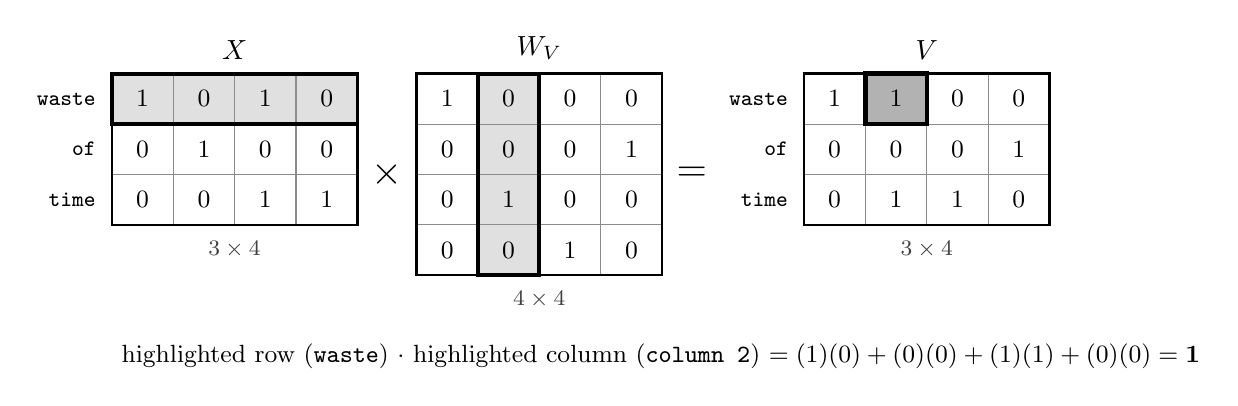
\begin{tikzpicture}
\draw[black!45, fill=black!12] (0.000,0.000) rectangle (0.780,-0.640);
\node[font=\small, text=black] at (0.390,-0.320) {$1$};
\draw[black!45, fill=black!12] (0.780,0.000) rectangle (1.560,-0.640);
\node[font=\small, text=black] at (1.170,-0.320) {$0$};
\draw[black!45, fill=black!12] (1.560,0.000) rectangle (2.340,-0.640);
\node[font=\small, text=black] at (1.950,-0.320) {$1$};
\draw[black!45, fill=black!12] (2.340,0.000) rectangle (3.120,-0.640);
\node[font=\small, text=black] at (2.730,-0.320) {$0$};
\draw[black!45, fill=white] (0.000,-0.640) rectangle (0.780,-1.279);
\node[font=\small, text=black] at (0.390,-0.959) {$0$};
\draw[black!45, fill=white] (0.780,-0.640) rectangle (1.560,-1.279);
\node[font=\small, text=black] at (1.170,-0.959) {$1$};
\draw[black!45, fill=white] (1.560,-0.640) rectangle (2.340,-1.279);
\node[font=\small, text=black] at (1.950,-0.959) {$0$};
\draw[black!45, fill=white] (2.340,-0.640) rectangle (3.120,-1.279);
\node[font=\small, text=black] at (2.730,-0.959) {$0$};
\draw[black!45, fill=white] (0.000,-1.279) rectangle (0.780,-1.919);
\node[font=\small, text=black] at (0.390,-1.599) {$0$};
\draw[black!45, fill=white] (0.780,-1.279) rectangle (1.560,-1.919);
\node[font=\small, text=black] at (1.170,-1.599) {$0$};
\draw[black!45, fill=white] (1.560,-1.279) rectangle (2.340,-1.919);
\node[font=\small, text=black] at (1.950,-1.599) {$1$};
\draw[black!45, fill=white] (2.340,-1.279) rectangle (3.120,-1.919);
\node[font=\small, text=black] at (2.730,-1.599) {$1$};
\draw[line width=1.4pt] (0.000,0.000) rectangle (3.120,-0.640);
\draw[line width=0.9pt] (0.000,0.000) rectangle (3.120,-1.919);
\node[anchor=east, font=\footnotesize\ttfamily] at (-0.080,-0.320) {waste};
\node[anchor=east, font=\footnotesize\ttfamily] at (-0.080,-0.959) {of};
\node[anchor=east, font=\footnotesize\ttfamily] at (-0.080,-1.599) {time};
\node[anchor=south, font=\normalsize] at (1.560,0.050) {$X$};
\node[anchor=north, font=\footnotesize, text=black!75] at (1.560,-1.999) {$3\times4$};
\draw[black!45, fill=white] (3.870,0.000) rectangle (4.650,-0.640);
\node[font=\small, text=black] at (4.260,-0.320) {$1$};
\draw[black!45, fill=black!12] (4.650,0.000) rectangle (5.430,-0.640);
\node[font=\small, text=black] at (5.040,-0.320) {$0$};
\draw[black!45, fill=white] (5.430,0.000) rectangle (6.210,-0.640);
\node[font=\small, text=black] at (5.820,-0.320) {$0$};
\draw[black!45, fill=white] (6.210,0.000) rectangle (6.990,-0.640);
\node[font=\small, text=black] at (6.600,-0.320) {$0$};
\draw[black!45, fill=white] (3.870,-0.640) rectangle (4.650,-1.279);
\node[font=\small, text=black] at (4.260,-0.959) {$0$};
\draw[black!45, fill=black!12] (4.650,-0.640) rectangle (5.430,-1.279);
\node[font=\small, text=black] at (5.040,-0.959) {$0$};
\draw[black!45, fill=white] (5.430,-0.640) rectangle (6.210,-1.279);
\node[font=\small, text=black] at (5.820,-0.959) {$0$};
\draw[black!45, fill=white] (6.210,-0.640) rectangle (6.990,-1.279);
\node[font=\small, text=black] at (6.600,-0.959) {$1$};
\draw[black!45, fill=white] (3.870,-1.279) rectangle (4.650,-1.919);
\node[font=\small, text=black] at (4.260,-1.599) {$0$};
\draw[black!45, fill=black!12] (4.650,-1.279) rectangle (5.430,-1.919);
\node[font=\small, text=black] at (5.040,-1.599) {$1$};
\draw[black!45, fill=white] (5.430,-1.279) rectangle (6.210,-1.919);
\node[font=\small, text=black] at (5.820,-1.599) {$0$};
\draw[black!45, fill=white] (6.210,-1.279) rectangle (6.990,-1.919);
\node[font=\small, text=black] at (6.600,-1.599) {$0$};
\draw[black!45, fill=white] (3.870,-1.919) rectangle (4.650,-2.558);
\node[font=\small, text=black] at (4.260,-2.239) {$0$};
\draw[black!45, fill=black!12] (4.650,-1.919) rectangle (5.430,-2.558);
\node[font=\small, text=black] at (5.040,-2.239) {$0$};
\draw[black!45, fill=white] (5.430,-1.919) rectangle (6.210,-2.558);
\node[font=\small, text=black] at (5.820,-2.239) {$1$};
\draw[black!45, fill=white] (6.210,-1.919) rectangle (6.990,-2.558);
\node[font=\small, text=black] at (6.600,-2.239) {$0$};
\draw[line width=1.4pt] (4.650,0.000) rectangle (5.430,-2.558);
\draw[line width=0.9pt] (3.870,0.000) rectangle (6.990,-2.558);
\node[anchor=south, font=\normalsize] at (5.430,0.050) {$W_V$};
\node[anchor=north, font=\footnotesize, text=black!75] at (5.430,-2.638) {$4\times4$};
\draw[black!45, fill=white] (8.790,0.000) rectangle (9.570,-0.640);
\node[font=\small, text=black] at (9.180,-0.320) {$1$};
\draw[black!45, fill=black!30] (9.570,0.000) rectangle (10.350,-0.640);
\node[font=\small, text=black] at (9.960,-0.320) {$1$};
\draw[black!45, fill=white] (10.350,0.000) rectangle (11.130,-0.640);
\node[font=\small, text=black] at (10.740,-0.320) {$0$};
\draw[black!45, fill=white] (11.130,0.000) rectangle (11.910,-0.640);
\node[font=\small, text=black] at (11.520,-0.320) {$0$};
\draw[black!45, fill=white] (8.790,-0.640) rectangle (9.570,-1.279);
\node[font=\small, text=black] at (9.180,-0.959) {$0$};
\draw[black!45, fill=white] (9.570,-0.640) rectangle (10.350,-1.279);
\node[font=\small, text=black] at (9.960,-0.959) {$0$};
\draw[black!45, fill=white] (10.350,-0.640) rectangle (11.130,-1.279);
\node[font=\small, text=black] at (10.740,-0.959) {$0$};
\draw[black!45, fill=white] (11.130,-0.640) rectangle (11.910,-1.279);
\node[font=\small, text=black] at (11.520,-0.959) {$1$};
\draw[black!45, fill=white] (8.790,-1.279) rectangle (9.570,-1.919);
\node[font=\small, text=black] at (9.180,-1.599) {$0$};
\draw[black!45, fill=white] (9.570,-1.279) rectangle (10.350,-1.919);
\node[font=\small, text=black] at (9.960,-1.599) {$1$};
\draw[black!45, fill=white] (10.350,-1.279) rectangle (11.130,-1.919);
\node[font=\small, text=black] at (10.740,-1.599) {$1$};
\draw[black!45, fill=white] (11.130,-1.279) rectangle (11.910,-1.919);
\node[font=\small, text=black] at (11.520,-1.599) {$0$};
\draw[line width=1.6pt] (9.570,0.000) rectangle (10.350,-0.640);
\draw[line width=0.9pt] (8.790,0.000) rectangle (11.910,-1.919);
\node[anchor=east, font=\footnotesize\ttfamily] at (8.710,-0.320) {waste};
\node[anchor=east, font=\footnotesize\ttfamily] at (8.710,-0.959) {of};
\node[anchor=east, font=\footnotesize\ttfamily] at (8.710,-1.599) {time};
\node[anchor=south, font=\normalsize] at (10.350,0.050) {$V$};
\node[anchor=north, font=\footnotesize, text=black!75] at (10.350,-1.999) {$3\times4$};
\node[font=\Large] at (3.495,-1.279) {$\times$};
\node[font=\Large] at (7.365,-1.279) {$=$};
\node[anchor=north west, font=\small, align=left] at (0,-3.308) {highlighted row (\texttt{waste}) $\cdot$ highlighted column (\texttt{column 2}) $= (1)(0) + (0)(0) + (1)(1) + (0)(0) = \mathbf{1}$};
\end{tikzpicture}

\caption{The three machines applied to the whole sentence: $Q=XW_Q$, $K=XW_K$, $V=XW_V$, each of shape
$T\times d_k=3\times4$. $W_Q$ is the identity in the toy, so $Q=X$; $W_K$ and $W_V$ move the arrows.}
\label{fig:qkv}
\end{figure}

\begin{checkq}
Why does attention give each token three arrows instead of one?
\begin{options}
\item It does not need to: the three are copies, and one would do.
\item What a token looks for, what it can be found by and what it hands over are different jobs, so each gets its own machine.
\item The values must keep the original meaning, so they cannot be shared with queries.
\item Only the current token needs a query; keys and values are for the other tokens.
\end{options}
\end{checkq}

\Summary{Each token gets a query (what it looks for), a key (what it is found by) and a value (what it hands over),
each from its own learned machine.}

%---------------------------------------------------------------------
\subsection*{3.6\quad Worked example: what does \tok{time} attend to?}

\Predict Look at $Q$ and $K$ above. Which earlier token do you expect \tok{time} to attend to most, and roughly
what share? Write it down before reading on.

\textbf{Step 1: match (every handshake at once).} $S = QK^\top$: every row of $Q$ meets every column of $K^\top$.
The highlighted row \tok{time} meeting the highlighted column \tok{waste} gives the cell circled in $S$.

\begin{figure}[!htb]
\centering
% AUTO-GENERATED by code/figlib.py helpers -- do not edit
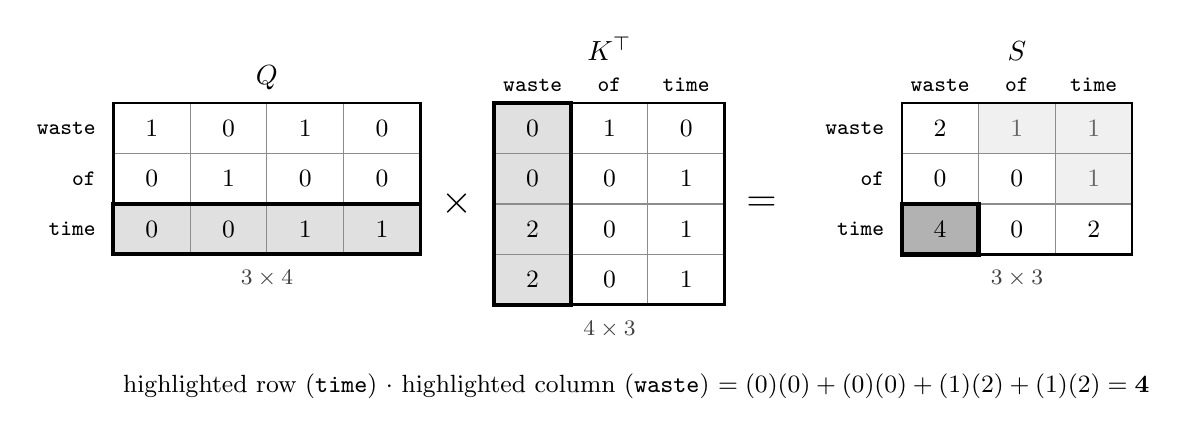
\begin{tikzpicture}[x=1.25cm]
\draw[black!45, fill=white] (0.000,0.000) rectangle (0.780,-0.640);
\node[font=\small, text=black] at (0.390,-0.320) {$1$};
\draw[black!45, fill=white] (0.780,0.000) rectangle (1.560,-0.640);
\node[font=\small, text=black] at (1.170,-0.320) {$0$};
\draw[black!45, fill=white] (1.560,0.000) rectangle (2.340,-0.640);
\node[font=\small, text=black] at (1.950,-0.320) {$1$};
\draw[black!45, fill=white] (2.340,0.000) rectangle (3.120,-0.640);
\node[font=\small, text=black] at (2.730,-0.320) {$0$};
\draw[black!45, fill=white] (0.000,-0.640) rectangle (0.780,-1.279);
\node[font=\small, text=black] at (0.390,-0.959) {$0$};
\draw[black!45, fill=white] (0.780,-0.640) rectangle (1.560,-1.279);
\node[font=\small, text=black] at (1.170,-0.959) {$1$};
\draw[black!45, fill=white] (1.560,-0.640) rectangle (2.340,-1.279);
\node[font=\small, text=black] at (1.950,-0.959) {$0$};
\draw[black!45, fill=white] (2.340,-0.640) rectangle (3.120,-1.279);
\node[font=\small, text=black] at (2.730,-0.959) {$0$};
\draw[black!45, fill=black!12] (0.000,-1.279) rectangle (0.780,-1.919);
\node[font=\small, text=black] at (0.390,-1.599) {$0$};
\draw[black!45, fill=black!12] (0.780,-1.279) rectangle (1.560,-1.919);
\node[font=\small, text=black] at (1.170,-1.599) {$0$};
\draw[black!45, fill=black!12] (1.560,-1.279) rectangle (2.340,-1.919);
\node[font=\small, text=black] at (1.950,-1.599) {$1$};
\draw[black!45, fill=black!12] (2.340,-1.279) rectangle (3.120,-1.919);
\node[font=\small, text=black] at (2.730,-1.599) {$1$};
\draw[line width=1.4pt] (0.000,-1.279) rectangle (3.120,-1.919);
\draw[line width=0.9pt] (0.000,0.000) rectangle (3.120,-1.919);
\node[anchor=east, font=\footnotesize\ttfamily] at (-0.080,-0.320) {waste};
\node[anchor=east, font=\footnotesize\ttfamily] at (-0.080,-0.959) {of};
\node[anchor=east, font=\footnotesize\ttfamily] at (-0.080,-1.599) {time};
\node[anchor=south, font=\normalsize] at (1.560,0.050) {$Q$};
\node[anchor=north, font=\footnotesize, text=black!75] at (1.560,-1.999) {$3\times4$};
\draw[black!45, fill=black!12] (3.870,0.000) rectangle (4.650,-0.640);
\node[font=\small, text=black] at (4.260,-0.320) {$0$};
\draw[black!45, fill=white] (4.650,0.000) rectangle (5.430,-0.640);
\node[font=\small, text=black] at (5.040,-0.320) {$1$};
\draw[black!45, fill=white] (5.430,0.000) rectangle (6.210,-0.640);
\node[font=\small, text=black] at (5.820,-0.320) {$0$};
\draw[black!45, fill=black!12] (3.870,-0.640) rectangle (4.650,-1.279);
\node[font=\small, text=black] at (4.260,-0.959) {$0$};
\draw[black!45, fill=white] (4.650,-0.640) rectangle (5.430,-1.279);
\node[font=\small, text=black] at (5.040,-0.959) {$0$};
\draw[black!45, fill=white] (5.430,-0.640) rectangle (6.210,-1.279);
\node[font=\small, text=black] at (5.820,-0.959) {$1$};
\draw[black!45, fill=black!12] (3.870,-1.279) rectangle (4.650,-1.919);
\node[font=\small, text=black] at (4.260,-1.599) {$2$};
\draw[black!45, fill=white] (4.650,-1.279) rectangle (5.430,-1.919);
\node[font=\small, text=black] at (5.040,-1.599) {$0$};
\draw[black!45, fill=white] (5.430,-1.279) rectangle (6.210,-1.919);
\node[font=\small, text=black] at (5.820,-1.599) {$1$};
\draw[black!45, fill=black!12] (3.870,-1.919) rectangle (4.650,-2.558);
\node[font=\small, text=black] at (4.260,-2.239) {$2$};
\draw[black!45, fill=white] (4.650,-1.919) rectangle (5.430,-2.558);
\node[font=\small, text=black] at (5.040,-2.239) {$0$};
\draw[black!45, fill=white] (5.430,-1.919) rectangle (6.210,-2.558);
\node[font=\small, text=black] at (5.820,-2.239) {$1$};
\draw[line width=1.4pt] (3.870,0.000) rectangle (4.650,-2.558);
\draw[line width=0.9pt] (3.870,0.000) rectangle (6.210,-2.558);
\node[anchor=south, font=\footnotesize\ttfamily] at (4.260,0.020) {waste};
\node[anchor=south, font=\footnotesize\ttfamily] at (5.040,0.020) {of};
\node[anchor=south, font=\footnotesize\ttfamily] at (5.820,0.020) {time};
\node[anchor=south, font=\normalsize] at (5.040,0.420) {$K^{\top}$};
\node[anchor=north, font=\footnotesize, text=black!75] at (5.040,-2.638) {$4\times3$};
\draw[black!45, fill=white] (8.010,0.000) rectangle (8.790,-0.640);
\node[font=\small, text=black] at (8.400,-0.320) {$2$};
\draw[black!45, fill=black!6] (8.790,0.000) rectangle (9.570,-0.640);
\node[font=\small, text=black!60] at (9.180,-0.320) {$1$};
\draw[black!45, fill=black!6] (9.570,0.000) rectangle (10.350,-0.640);
\node[font=\small, text=black!60] at (9.960,-0.320) {$1$};
\draw[black!45, fill=white] (8.010,-0.640) rectangle (8.790,-1.279);
\node[font=\small, text=black] at (8.400,-0.959) {$0$};
\draw[black!45, fill=white] (8.790,-0.640) rectangle (9.570,-1.279);
\node[font=\small, text=black] at (9.180,-0.959) {$0$};
\draw[black!45, fill=black!6] (9.570,-0.640) rectangle (10.350,-1.279);
\node[font=\small, text=black!60] at (9.960,-0.959) {$1$};
\draw[black!45, fill=black!30] (8.010,-1.279) rectangle (8.790,-1.919);
\node[font=\small, text=black] at (8.400,-1.599) {$4$};
\draw[black!45, fill=white] (8.790,-1.279) rectangle (9.570,-1.919);
\node[font=\small, text=black] at (9.180,-1.599) {$0$};
\draw[black!45, fill=white] (9.570,-1.279) rectangle (10.350,-1.919);
\node[font=\small, text=black] at (9.960,-1.599) {$2$};
\draw[line width=1.6pt] (8.010,-1.279) rectangle (8.790,-1.919);
\draw[line width=0.9pt] (8.010,0.000) rectangle (10.350,-1.919);
\node[anchor=east, font=\footnotesize\ttfamily] at (7.930,-0.320) {waste};
\node[anchor=east, font=\footnotesize\ttfamily] at (7.930,-0.959) {of};
\node[anchor=east, font=\footnotesize\ttfamily] at (7.930,-1.599) {time};
\node[anchor=south, font=\footnotesize\ttfamily] at (8.400,0.020) {waste};
\node[anchor=south, font=\footnotesize\ttfamily] at (9.180,0.020) {of};
\node[anchor=south, font=\footnotesize\ttfamily] at (9.960,0.020) {time};
\node[anchor=south, font=\normalsize] at (9.180,0.420) {$S$};
\node[anchor=north, font=\footnotesize, text=black!75] at (9.180,-1.999) {$3\times3$};
\node[font=\Large] at (3.495,-1.279) {$\times$};
\node[font=\Large] at (6.585,-1.279) {$=$};
\node[anchor=north west, font=\small, align=left] at (0,-3.308) {highlighted row (\texttt{time}) $\cdot$ highlighted column (\texttt{waste}) $= (0)(0) + (0)(0) + (1)(2) + (1)(2) = \mathbf{4}$};
\end{tikzpicture}

\caption{$S=QK^\top$ for our sentence, $(3\times4)(4\times3)=3\times3$. Row \tok{time} reads $(\sWaste, \sOf,
\sTime)$. Grey cells are a token meeting a token that comes \emph{after} it; Step 3 removes them.}
\end{figure}

Look at row \tok{time} through the geometry of \S3.2. Its query is $\bm{q}_{\text{time}}=(0,0,1,1)$, of length
\lenQ. Each score is length $\times$ length $\times$ agreement:

\begin{center}
\small
\begin{tabular}{@{}l c c c c c@{}}
\toprule
key & $\lVert\bm{k}\rVert$ & angle to $\bm{q}_{\text{time}}$ & $\cos\theta$ & $\lVert\bm{q}\rVert\lVert\bm{k}\rVert\cos\theta$ & dot product\\
\midrule
\tok{waste} & \lenWaste & \angWaste$^\circ$ & \cosWaste & \sWaste & \sWaste\\
\tok{of} & \lenOf & \angOf$^\circ$ & \cosOf & \sOf & \sOf\\
\tok{time} & \lenTime & \angTime$^\circ$ & \cosTime & \sTime & \sTime\\
\bottomrule
\end{tabular}
\end{center}
\tok{time}'s question points \emph{exactly} along \tok{waste}'s label (0 degrees), at right angles to \tok{of}'s
(nothing in common), and partly along its own. That is what ``\tok{waste} is relevant to \tok{time}'' means,
geometrically.

\textbf{Step 2: scale.} Divide by $\sqrt{d_k}=\sqrt4=2$. Row \tok{time} becomes $(\ssWaste, \ssOf, \ssTime)$. Why
we divide is the subject of \S3.8.

\textbf{Step 3: cover the answers.} Remember from \S1.9 that one sentence is three exercises: after \tok{waste},
guess the next word; after \tok{waste of}, guess the next; and so on. The exercise ``after \tok{waste of}, guess
the next word'' must not be allowed to see \tok{time}: that is the answer.

\Picture An exam where all the questions and all the answers are printed on one long sheet, in order. Before each
question, you cover everything below it with a ruler. A fraud-detection model is trained the same way: it may
never use information recorded \emph{after} the transaction, because in production that information does not
exist yet. A model that used it would look brilliant in training and fail in the real world.

\begin{breaks}
On the exam sheet you cover the answers once. Here every row has its own ruler at a different height, and all the
rulers are applied at the same moment.
\end{breaks}

\Exactly Set every score above the diagonal (the grey cells) to $-\infty$. This is \emph{causal masking}:
\begin{center}% AUTO-GENERATED by code/figlib.py helpers -- do not edit
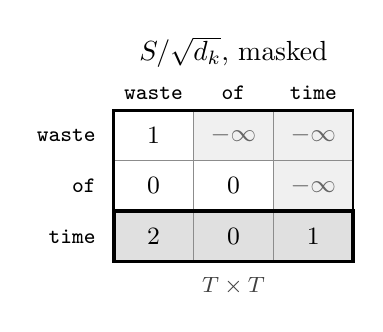
\begin{tikzpicture}[x=1.3cm]
\draw[black!45, fill=white] (0.000,0.000) rectangle (0.780,-0.640);
\node[font=\small, text=black] at (0.390,-0.320) {$1$};
\draw[black!45, fill=black!6] (0.780,0.000) rectangle (1.560,-0.640);
\node[font=\small, text=black!60] at (1.170,-0.320) {$-\infty$};
\draw[black!45, fill=black!6] (1.560,0.000) rectangle (2.340,-0.640);
\node[font=\small, text=black!60] at (1.950,-0.320) {$-\infty$};
\draw[black!45, fill=white] (0.000,-0.640) rectangle (0.780,-1.279);
\node[font=\small, text=black] at (0.390,-0.959) {$0$};
\draw[black!45, fill=white] (0.780,-0.640) rectangle (1.560,-1.279);
\node[font=\small, text=black] at (1.170,-0.959) {$0$};
\draw[black!45, fill=black!6] (1.560,-0.640) rectangle (2.340,-1.279);
\node[font=\small, text=black!60] at (1.950,-0.959) {$-\infty$};
\draw[black!45, fill=black!12] (0.000,-1.279) rectangle (0.780,-1.919);
\node[font=\small, text=black] at (0.390,-1.599) {$2$};
\draw[black!45, fill=black!12] (0.780,-1.279) rectangle (1.560,-1.919);
\node[font=\small, text=black] at (1.170,-1.599) {$0$};
\draw[black!45, fill=black!12] (1.560,-1.279) rectangle (2.340,-1.919);
\node[font=\small, text=black] at (1.950,-1.599) {$1$};
\draw[line width=1.4pt] (0.000,-1.279) rectangle (2.340,-1.919);
\draw[line width=0.9pt] (0.000,0.000) rectangle (2.340,-1.919);
\node[anchor=east, font=\footnotesize\ttfamily] at (-0.080,-0.320) {waste};
\node[anchor=east, font=\footnotesize\ttfamily] at (-0.080,-0.959) {of};
\node[anchor=east, font=\footnotesize\ttfamily] at (-0.080,-1.599) {time};
\node[anchor=south, font=\footnotesize\ttfamily] at (0.390,0.020) {waste};
\node[anchor=south, font=\footnotesize\ttfamily] at (1.170,0.020) {of};
\node[anchor=south, font=\footnotesize\ttfamily] at (1.950,0.020) {time};
\node[anchor=south, font=\normalsize] at (1.170,0.420) {$S/\sqrt{d_k}$, masked};
\node[anchor=north, font=\footnotesize, text=black!75] at (1.170,-1.999) {$T\times T$};
\end{tikzpicture}
\end{center}
Step 4 will turn $-\infty$ into a weight of exactly zero. So the row for \tok{of} is built only from \tok{waste}
and \tok{of}; our script checks that changing the arrow of \tok{time} to anything at all leaves the first two rows
of the output untouched. That is why the three exercises can be solved \emph{in the same pass} without cheating.

\begin{wrongidea}{3.7}
\emph{The mask exists only to stop cheating.} That is how it is usually introduced: without it, the model
could copy from the future tokens. That is true, and it is half the story. The other half
is speed: because each row ignores everything after it, one pass can train all $T$ positions at once. Without
the mask you would need $T$ separate passes, one per prefix.
\end{wrongidea}

\textbf{Step 4: turn scores into shares (softmax).} For each row: raise $e$ to each score, then divide by the
row's total. For \tok{time}, the three steps are the three rows of this table:
\begin{center}% AUTO-GENERATED by code/figlib.py helpers -- do not edit
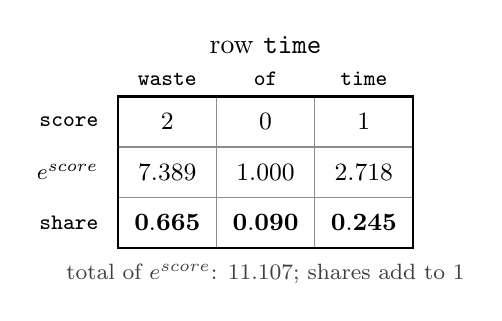
\begin{tikzpicture}[x=1.6cm]
\draw[black!45, fill=white] (0.000,0.000) rectangle (0.780,-0.640);
\node[font=\small, text=black] at (0.390,-0.320) {$2$};
\draw[black!45, fill=white] (0.780,0.000) rectangle (1.560,-0.640);
\node[font=\small, text=black] at (1.170,-0.320) {$0$};
\draw[black!45, fill=white] (1.560,0.000) rectangle (2.340,-0.640);
\node[font=\small, text=black] at (1.950,-0.320) {$1$};
\draw[black!45, fill=white] (0.000,-0.640) rectangle (0.780,-1.279);
\node[font=\small, text=black] at (0.390,-0.959) {$7.389$};
\draw[black!45, fill=white] (0.780,-0.640) rectangle (1.560,-1.279);
\node[font=\small, text=black] at (1.170,-0.959) {$1.000$};
\draw[black!45, fill=white] (1.560,-0.640) rectangle (2.340,-1.279);
\node[font=\small, text=black] at (1.950,-0.959) {$2.718$};
\draw[black!45, fill=white] (0.000,-1.279) rectangle (0.780,-1.919);
\node[font=\small, text=black] at (0.390,-1.599) {$\mathbf{0.665}$};
\draw[black!45, fill=white] (0.780,-1.279) rectangle (1.560,-1.919);
\node[font=\small, text=black] at (1.170,-1.599) {$\mathbf{0.090}$};
\draw[black!45, fill=white] (1.560,-1.279) rectangle (2.340,-1.919);
\node[font=\small, text=black] at (1.950,-1.599) {$\mathbf{0.245}$};
\draw[line width=0.9pt] (0.000,0.000) rectangle (2.340,-1.919);
\node[anchor=east, font=\footnotesize\ttfamily] at (-0.080,-0.320) {score};
\node[anchor=east, font=\footnotesize\ttfamily] at (-0.080,-0.959) {$e^{\text{score}}$};
\node[anchor=east, font=\footnotesize\ttfamily] at (-0.080,-1.599) {share};
\node[anchor=south, font=\footnotesize\ttfamily] at (0.390,0.020) {waste};
\node[anchor=south, font=\footnotesize\ttfamily] at (1.170,0.020) {of};
\node[anchor=south, font=\footnotesize\ttfamily] at (1.950,0.020) {time};
\node[anchor=south, font=\normalsize] at (1.170,0.420) {row \texttt{time}};
\node[anchor=north, font=\footnotesize, text=black!75] at (1.170,-1.999) {total of $e^{\text{score}}$: $11.107$; shares add to 1};
\end{tikzpicture}
\end{center}
In symbols, $\bm{a}_{\text{time}} = \left(\tfrac{\eWaste}{\eSum},\ \tfrac{\eOf}{\eSum},\ \tfrac{\eTime}{\eSum}\right)
= (\aWaste,\ \aOf,\ \aTime)$.
\tok{time} gives \apctWaste\% of its attention to \tok{waste}, \apctOf\% to \tok{of} and \apctTime\% to itself.
How close was your prediction? Compare that with the fixed 33.3\% each of \S3.1: the weights now come from the
content.

\Sanity The three shares are positive and add to 1, and the biggest score got the biggest share. A share above 1
or a negative share would mean an arithmetic slip.

\begin{wrongidea}{3.2}
\emph{Attention scores are already percentages.} They come out as one number per pair, like a table of shares, so
it is natural to read $(\sWaste,\sOf,\sTime)$ as ``4 parts to \tok{waste}''. No: scores can be negative and do not add to 1. Only after
softmax are they shares.
\end{wrongidea}

\begin{wrongidea}{3.5}
\emph{The current token only needs a query; keys and values are for the other tokens.} The current token is the
one asking, so its own key and value seem pointless.
Look at the result: \tok{time} gives \apctTime\% of its attention to \emph{itself}, through its own key and value.
And later tokens, such as \tok{Sorry}, will look back at \tok{time} through the same key and value.
\end{wrongidea}

\textbf{Step 5: collect.} The shares are shares \emph{of the values}, the contents of the books:
\[
\bm{o}_{\text{time}} = \aWaste\,\bm{v}_{\text{waste}} + \aOf\,\bm{v}_{\text{of}} + \aTime\,\bm{v}_{\text{time}}
= \oTime \shape{1\times d_k}
\]
and for the whole sentence at once, $O=AV$ ($T\times T$ times $T\times d_k$). The highlighted row of $A$ holds
\tok{time}'s shares; the highlighted column of $V$ holds the second number of each value arrow:
\begin{center}\resizebox{\linewidth}{!}{% AUTO-GENERATED by code/figlib.py helpers -- do not edit
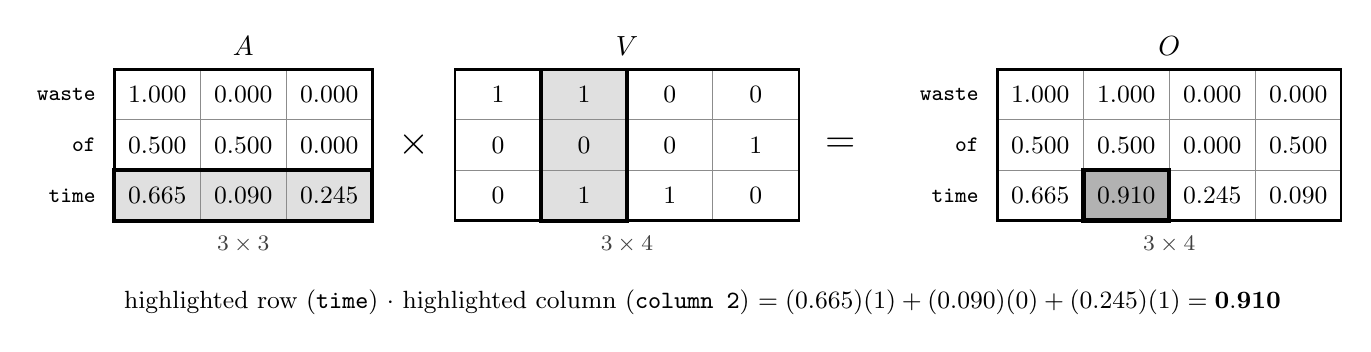
\begin{tikzpicture}[x=1.4cm]
\draw[black!45, fill=white] (0.000,0.000) rectangle (0.780,-0.640);
\node[font=\small, text=black] at (0.390,-0.320) {$1.000$};
\draw[black!45, fill=white] (0.780,0.000) rectangle (1.560,-0.640);
\node[font=\small, text=black] at (1.170,-0.320) {$0.000$};
\draw[black!45, fill=white] (1.560,0.000) rectangle (2.340,-0.640);
\node[font=\small, text=black] at (1.950,-0.320) {$0.000$};
\draw[black!45, fill=white] (0.000,-0.640) rectangle (0.780,-1.279);
\node[font=\small, text=black] at (0.390,-0.959) {$0.500$};
\draw[black!45, fill=white] (0.780,-0.640) rectangle (1.560,-1.279);
\node[font=\small, text=black] at (1.170,-0.959) {$0.500$};
\draw[black!45, fill=white] (1.560,-0.640) rectangle (2.340,-1.279);
\node[font=\small, text=black] at (1.950,-0.959) {$0.000$};
\draw[black!45, fill=black!12] (0.000,-1.279) rectangle (0.780,-1.919);
\node[font=\small, text=black] at (0.390,-1.599) {$0.665$};
\draw[black!45, fill=black!12] (0.780,-1.279) rectangle (1.560,-1.919);
\node[font=\small, text=black] at (1.170,-1.599) {$0.090$};
\draw[black!45, fill=black!12] (1.560,-1.279) rectangle (2.340,-1.919);
\node[font=\small, text=black] at (1.950,-1.599) {$0.245$};
\draw[line width=1.4pt] (0.000,-1.279) rectangle (2.340,-1.919);
\draw[line width=0.9pt] (0.000,0.000) rectangle (2.340,-1.919);
\node[anchor=east, font=\footnotesize\ttfamily] at (-0.080,-0.320) {waste};
\node[anchor=east, font=\footnotesize\ttfamily] at (-0.080,-0.959) {of};
\node[anchor=east, font=\footnotesize\ttfamily] at (-0.080,-1.599) {time};
\node[anchor=south, font=\normalsize] at (1.170,0.050) {$A$};
\node[anchor=north, font=\footnotesize, text=black!75] at (1.170,-1.999) {$3\times3$};
\draw[black!45, fill=white] (3.090,0.000) rectangle (3.870,-0.640);
\node[font=\small, text=black] at (3.480,-0.320) {$1$};
\draw[black!45, fill=black!12] (3.870,0.000) rectangle (4.650,-0.640);
\node[font=\small, text=black] at (4.260,-0.320) {$1$};
\draw[black!45, fill=white] (4.650,0.000) rectangle (5.430,-0.640);
\node[font=\small, text=black] at (5.040,-0.320) {$0$};
\draw[black!45, fill=white] (5.430,0.000) rectangle (6.210,-0.640);
\node[font=\small, text=black] at (5.820,-0.320) {$0$};
\draw[black!45, fill=white] (3.090,-0.640) rectangle (3.870,-1.279);
\node[font=\small, text=black] at (3.480,-0.959) {$0$};
\draw[black!45, fill=black!12] (3.870,-0.640) rectangle (4.650,-1.279);
\node[font=\small, text=black] at (4.260,-0.959) {$0$};
\draw[black!45, fill=white] (4.650,-0.640) rectangle (5.430,-1.279);
\node[font=\small, text=black] at (5.040,-0.959) {$0$};
\draw[black!45, fill=white] (5.430,-0.640) rectangle (6.210,-1.279);
\node[font=\small, text=black] at (5.820,-0.959) {$1$};
\draw[black!45, fill=white] (3.090,-1.279) rectangle (3.870,-1.919);
\node[font=\small, text=black] at (3.480,-1.599) {$0$};
\draw[black!45, fill=black!12] (3.870,-1.279) rectangle (4.650,-1.919);
\node[font=\small, text=black] at (4.260,-1.599) {$1$};
\draw[black!45, fill=white] (4.650,-1.279) rectangle (5.430,-1.919);
\node[font=\small, text=black] at (5.040,-1.599) {$1$};
\draw[black!45, fill=white] (5.430,-1.279) rectangle (6.210,-1.919);
\node[font=\small, text=black] at (5.820,-1.599) {$0$};
\draw[line width=1.4pt] (3.870,0.000) rectangle (4.650,-1.919);
\draw[line width=0.9pt] (3.090,0.000) rectangle (6.210,-1.919);
\node[anchor=south, font=\normalsize] at (4.650,0.050) {$V$};
\node[anchor=north, font=\footnotesize, text=black!75] at (4.650,-1.999) {$3\times4$};
\draw[black!45, fill=white] (8.010,0.000) rectangle (8.790,-0.640);
\node[font=\small, text=black] at (8.400,-0.320) {$1.000$};
\draw[black!45, fill=white] (8.790,0.000) rectangle (9.570,-0.640);
\node[font=\small, text=black] at (9.180,-0.320) {$1.000$};
\draw[black!45, fill=white] (9.570,0.000) rectangle (10.350,-0.640);
\node[font=\small, text=black] at (9.960,-0.320) {$0.000$};
\draw[black!45, fill=white] (10.350,0.000) rectangle (11.130,-0.640);
\node[font=\small, text=black] at (10.740,-0.320) {$0.000$};
\draw[black!45, fill=white] (8.010,-0.640) rectangle (8.790,-1.279);
\node[font=\small, text=black] at (8.400,-0.959) {$0.500$};
\draw[black!45, fill=white] (8.790,-0.640) rectangle (9.570,-1.279);
\node[font=\small, text=black] at (9.180,-0.959) {$0.500$};
\draw[black!45, fill=white] (9.570,-0.640) rectangle (10.350,-1.279);
\node[font=\small, text=black] at (9.960,-0.959) {$0.000$};
\draw[black!45, fill=white] (10.350,-0.640) rectangle (11.130,-1.279);
\node[font=\small, text=black] at (10.740,-0.959) {$0.500$};
\draw[black!45, fill=white] (8.010,-1.279) rectangle (8.790,-1.919);
\node[font=\small, text=black] at (8.400,-1.599) {$0.665$};
\draw[black!45, fill=black!30] (8.790,-1.279) rectangle (9.570,-1.919);
\node[font=\small, text=black] at (9.180,-1.599) {$0.910$};
\draw[black!45, fill=white] (9.570,-1.279) rectangle (10.350,-1.919);
\node[font=\small, text=black] at (9.960,-1.599) {$0.245$};
\draw[black!45, fill=white] (10.350,-1.279) rectangle (11.130,-1.919);
\node[font=\small, text=black] at (10.740,-1.599) {$0.090$};
\draw[line width=1.6pt] (8.790,-1.279) rectangle (9.570,-1.919);
\draw[line width=0.9pt] (8.010,0.000) rectangle (11.130,-1.919);
\node[anchor=east, font=\footnotesize\ttfamily] at (7.930,-0.320) {waste};
\node[anchor=east, font=\footnotesize\ttfamily] at (7.930,-0.959) {of};
\node[anchor=east, font=\footnotesize\ttfamily] at (7.930,-1.599) {time};
\node[anchor=south, font=\normalsize] at (9.570,0.050) {$O$};
\node[anchor=north, font=\footnotesize, text=black!75] at (9.570,-1.999) {$3\times4$};
\node[font=\Large] at (2.715,-0.959) {$\times$};
\node[font=\Large] at (6.585,-0.959) {$=$};
\node[anchor=north west, font=\small, align=left] at (0,-2.669) {highlighted row (\texttt{time}) $\cdot$ highlighted column (\texttt{column 2}) $= (0.665)(1) + (0.090)(0) + (0.245)(1) = \mathbf{0.910}$};
\end{tikzpicture}
}\end{center}
Every row of $O$ is a blend of value arrows, mixed in the proportions the token asked for. The arrow of \tok{time}
that leaves this step is no longer ``time in general''; it carries \apctWaste\% of what \tok{waste} had to say.

\begin{figure}[h]
\centering
\begin{tikzpicture}[x=0.47cm,y=0.47cm,font=\footnotesize]
\newcommand{\panel}[6]{%
  \begin{scope}[shift={(#1,0)}]
  \draw[gray!60] (-0.4,0)--(6.4,0);
  \fill[black!70] (0,0) rectangle (1.6,#3*#6);
  \fill[black!35] (2.2,0) rectangle (3.8,#4*#6);
  \fill[black!55] (4.4,0) rectangle (6.0,#5*#6);
  \node[above] at (0.8,#3*#6) {#3}; \node[above] at (3.0,#4*#6) {#4}; \node[above] at (5.2,#5*#6) {#5};
  \node at (3,-0.9) {#2};
  \end{scope}}
\panel{0}{1. match $S$}{\sWaste}{\sOf}{\sTime}{0.9}
\panel{9}{2. scale $\div\sqrt{d_k}$}{\ssWaste}{\ssOf}{\ssTime}{0.9}
\panel{18}{3--4a. exponentiate}{\eWaste}{\eOf}{\eTime}{0.5}
\panel{27}{4b. normalise}{\aWaste}{\aOf}{\aTime}{5}
\foreach \x in {7.3,16.3,25.3} \draw[-{Stealth},black!70, line width=0.8pt] (\x,2)--(\x+1.2,2);
\end{tikzpicture}
\caption{The frames of attention for the query \tok{time}. Bars: \tok{waste}, \tok{of}, \tok{time}. In the web
edition this strip is an animation you can scrub and re-run with your own weights.}
\end{figure}

\begin{checkq}
After masking, why can the three next-word exercises of \tok{waste of time} be trained in a single pass?
\begin{options}
\item The mask only stops cheating; it has nothing to do with doing them together.
\item Each row's output depends only on that token and earlier ones, so every row is an honest answer to its own exercise.
\item The raw scores are already percentages, so no extra step is needed per row.
\item Because \tok{time} gives no attention to itself.
\end{options}
\end{checkq}

\Summary{Match queries with keys, scale, mask the future, turn scores into shares, and blend the values: \tok{time}
ends up carrying \apctWaste\% of \tok{waste}.}

%---------------------------------------------------------------------
\subsection*{3.7\quad Why softmax, and not ``divide by the total''?}

\Picture A pizza is shared among friends according to votes. Softmax is the sharing rule.

\begin{breaks}
Votes are never negative, but scores can be. And the pizza rule we are about to build rewards a clear winner far
more than a fair-minded host would.
\end{breaks}

Three properties make $e^{\text{score}}$ the right rule, and each one is a requirement you could have written
down yourself:
\begin{enumerate}[label=(\roman*)]
\item \emph{Shares must be positive}, but scores can be negative (arrows pointing apart). $e^{s}$ is positive for
every $s$, and $e^{-\infty}=0$, which is what the mask needs.
\item \emph{Only differences should matter.} If every friend's vote goes up by 10, nobody deserves more pizza.
Indeed $e^{s+10}=e^{10}e^{s}$, and the common factor $e^{10}$ cancels in the division; our script confirms that
$(\ssWaste,\ssOf,\ssTime)$ and the same scores plus 10 give identical shares.
\item \emph{Leaders should lead.} Each extra point of score multiplies a share's weight by $e\approx2.718$, so a
clear winner gets a clear majority instead of a narrow one.
\end{enumerate}

\Predict Keep \tok{time}'s query pointing the same way but make it twice as long. Will the share for \tok{waste}
go up, go down, or stay at \aWaste?

Its scaled scores become $\dblScores$ and the shares become $(\dblWaste, \dblOf, \dblTime)$: same ranking, much
more decisive. \emph{The direction of a query decides what it looks for; its length decides how sure it is.}

\begin{wrongidea}{3.11}
\emph{Softmax shares depend on the ratios between scores, as when dividing by the total.} That is how percentages
are usually made, so it is the first rule anyone tries. Dividing by the total would give
$(\nThreeRatioA)$ for $(2,0,1)$ and $(\nThreeRatioB)$ for $(7,5,6)$: the shares would change when every score moves up by the same
amount. Softmax gives $(\nThreeSoft)$ for both, because of property (ii).
\end{wrongidea}

\begin{checkq}
After scaling, \tok{time}'s scores are $(2, 0, 1)$. Add 5 to all three, giving $(7, 5, 6)$, and apply softmax. What
happens to the shares? Then pick the reason.
\begin{options}
\item They do not change.
\item They all grow, because every score grew.
\item They become more even, since 7, 5 and 6 are closer together relative to their size.
\item \tok{waste}'s share grows most, because it had the largest score.
\end{options}
\emph{Reason:} (i) softmax only sees differences between scores; (ii) shares must still add to 1; (iii) $e^x$
grows faster for bigger $x$.
\end{checkq}

\Summary{Softmax makes shares that are positive, ignore a common shift, and favour the leader, and a longer query
makes it more decisive.}

%---------------------------------------------------------------------
\subsection*{3.8\quad Why divide by $\sqrt{d_k}$?}

In the toy the division looks cosmetic. It is not.

\Picture Toss a coin $d_k$ times; step forward on heads, back on tails. After 4 tosses you are usually within
about 2 steps of the start; after 1024 tosses, usually within about 32. The more tosses, the further you wander,
but not $d_k$ steps: about $\sqrt{d_k}$.

\begin{breaks}
Coin tosses are exactly $+1$ or $-1$. The products inside a dot product take any size; the $\sqrt{d_k}$ rule still
holds when each product has mean 0 and variance 1, which is how weights start out.
\end{breaks}

\Predict At $d_k=1024$, with no scaling, what share do you expect the top key to get out of 8 random keys, before
any training? Closer to $1/8$, to $1/2$, or to 1?

\Exactly A dot product of two unrelated arrows is a sum of $d_k$ products that are equally likely to be positive or
negative, like those coin tosses. If each coordinate has mean 0 and variance 1, the sum has variance $d_k$, so its
typical size is $\sqrt{d_k}$. We measured it (random queries against 8 random keys, 4000 trials, fixed seed):

\begin{center}
\small
\begin{tabular}{@{}r r r r@{}}
\toprule
$d_k$ & spread of $\bm{q}\cdot\bm{k}$ (theory $\sqrt{d_k}$) & largest share, unscaled & largest share, scaled\\
\midrule
4 & \sdFour\ (\sqrtFour) & \mxRawFour & \mxScFour\\
64 & \sdSixtyFour\ (\sqrtSixtyFour) & \mxRawSixtyFour & \mxScSixtyFour\\
1024 & \sdThousand\ (\sqrtThousand) & \mxRawThousand & \mxScThousand\\
\bottomrule
\end{tabular}
\end{center}

Read the third column with property (iii) of softmax in mind. At the widths real models use, random scores are tens
of points apart, so softmax hands almost everything to one key (\mxRawThousand\ on average at $d_k=1024$)
\emph{before the model has learned anything}. It has made up its mind at random, and, as Chapter 8 shows, a softmax
that has made up its mind barely responds to learning. Dividing by $\sqrt{d_k}$ shrinks the scores back to the size
of a one-step walk, and the starting shares stay spread (about \mxScThousand) at every width.

\Why A design rule you will meet again in Chapter 11: \emph{keep the size of every signal independent of the size of
the model}, so that making the model bigger does not silently change how it behaves.

\begin{wrongidea}{3.3}
\emph{Dividing by $\sqrt{d_k}$ normalises the vectors to length 1.} Cosine similarity divides by the lengths, and
the formula looks alike, so the two get merged. But $\sqrt{d_k}$ is one fixed number for the whole model; it does
not depend on any vector's length. It controls the \emph{spread} of scores across random pairs, not the length of
any one arrow. Lengths still matter after scaling, as \S3.7 showed.
\end{wrongidea}

\begin{checkq}
Why are attention scores divided by $\sqrt{d_k}$?
\begin{options}
\item To give every query and key length 1.
\item To keep the typical spread of scores near 1 at any width, so softmax does not pick a winner at random before training.
\item To turn the scores into percentages.
\item Because in the toy $\sqrt{d_k}=2$ makes the arithmetic tidy.
\end{options}
\end{checkq}

\Summary{Random dot products grow like $\sqrt{d_k}$, so dividing by it keeps softmax undecided at the start, at any
model width.}

%---------------------------------------------------------------------
\subsection*{3.9\quad Not one token, not one sentence: the whole batch at once}

We followed \tok{time} by hand, but the machine never handles one token. Look again at the shapes: $S=QK^\top$
computed every row at once. Now put a second customer reply in the same batch, \tok{not very useful}, with its own
arrows (rows of the same embedding table). The batch is two matrices stacked one behind the other, and so is
the table of scores:
\begin{figure}[!htb]\centering
% AUTO-GENERATED by code/figlib.py helpers -- do not edit
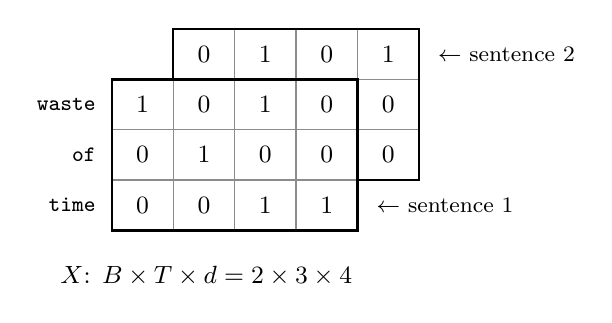
\begin{tikzpicture}
\fill[white] (0.780,0.640) rectangle (3.900,-1.279);
\draw[black!45, fill=white] (0.780,0.640) rectangle (1.560,0.000);
\node[font=\small, text=black] at (1.170,0.320) {$0$};
\draw[black!45, fill=white] (1.560,0.640) rectangle (2.340,0.000);
\node[font=\small, text=black] at (1.950,0.320) {$1$};
\draw[black!45, fill=white] (2.340,0.640) rectangle (3.120,0.000);
\node[font=\small, text=black] at (2.730,0.320) {$0$};
\draw[black!45, fill=white] (3.120,0.640) rectangle (3.900,0.000);
\node[font=\small, text=black] at (3.510,0.320) {$1$};
\draw[black!45, fill=white] (0.780,0.000) rectangle (1.560,-0.640);
\node[font=\small, text=black] at (1.170,-0.320) {$1$};
\draw[black!45, fill=white] (1.560,0.000) rectangle (2.340,-0.640);
\node[font=\small, text=black] at (1.950,-0.320) {$0$};
\draw[black!45, fill=white] (2.340,0.000) rectangle (3.120,-0.640);
\node[font=\small, text=black] at (2.730,-0.320) {$0$};
\draw[black!45, fill=white] (3.120,0.000) rectangle (3.900,-0.640);
\node[font=\small, text=black] at (3.510,-0.320) {$0$};
\draw[black!45, fill=white] (0.780,-0.640) rectangle (1.560,-1.279);
\node[font=\small, text=black] at (1.170,-0.959) {$0$};
\draw[black!45, fill=white] (1.560,-0.640) rectangle (2.340,-1.279);
\node[font=\small, text=black] at (1.950,-0.959) {$0$};
\draw[black!45, fill=white] (2.340,-0.640) rectangle (3.120,-1.279);
\node[font=\small, text=black] at (2.730,-0.959) {$1$};
\draw[black!45, fill=white] (3.120,-0.640) rectangle (3.900,-1.279);
\node[font=\small, text=black] at (3.510,-0.959) {$0$};
\draw[line width=0.9pt] (0.780,0.640) rectangle (3.900,-1.279);
\node[anchor=west, font=\footnotesize] at (4.020,0.320) {$\leftarrow$ sentence 2};
\fill[white] (0.000,0.000) rectangle (3.120,-1.919);
\draw[black!45, fill=white] (0.000,0.000) rectangle (0.780,-0.640);
\node[font=\small, text=black] at (0.390,-0.320) {$1$};
\draw[black!45, fill=white] (0.780,0.000) rectangle (1.560,-0.640);
\node[font=\small, text=black] at (1.170,-0.320) {$0$};
\draw[black!45, fill=white] (1.560,0.000) rectangle (2.340,-0.640);
\node[font=\small, text=black] at (1.950,-0.320) {$1$};
\draw[black!45, fill=white] (2.340,0.000) rectangle (3.120,-0.640);
\node[font=\small, text=black] at (2.730,-0.320) {$0$};
\draw[black!45, fill=white] (0.000,-0.640) rectangle (0.780,-1.279);
\node[font=\small, text=black] at (0.390,-0.959) {$0$};
\draw[black!45, fill=white] (0.780,-0.640) rectangle (1.560,-1.279);
\node[font=\small, text=black] at (1.170,-0.959) {$1$};
\draw[black!45, fill=white] (1.560,-0.640) rectangle (2.340,-1.279);
\node[font=\small, text=black] at (1.950,-0.959) {$0$};
\draw[black!45, fill=white] (2.340,-0.640) rectangle (3.120,-1.279);
\node[font=\small, text=black] at (2.730,-0.959) {$0$};
\draw[black!45, fill=white] (0.000,-1.279) rectangle (0.780,-1.919);
\node[font=\small, text=black] at (0.390,-1.599) {$0$};
\draw[black!45, fill=white] (0.780,-1.279) rectangle (1.560,-1.919);
\node[font=\small, text=black] at (1.170,-1.599) {$0$};
\draw[black!45, fill=white] (1.560,-1.279) rectangle (2.340,-1.919);
\node[font=\small, text=black] at (1.950,-1.599) {$1$};
\draw[black!45, fill=white] (2.340,-1.279) rectangle (3.120,-1.919);
\node[font=\small, text=black] at (2.730,-1.599) {$1$};
\draw[line width=0.9pt] (0.000,0.000) rectangle (3.120,-1.919);
\node[anchor=east, font=\footnotesize\ttfamily] at (-0.080,-0.320) {waste};
\node[anchor=east, font=\footnotesize\ttfamily] at (-0.080,-0.959) {of};
\node[anchor=east, font=\footnotesize\ttfamily] at (-0.080,-1.599) {time};
\node[anchor=west, font=\footnotesize] at (3.240,-1.599) {$\leftarrow$ sentence 1};
\node[anchor=north, font=\small] at (1.2,-2.25) {$X$: $B\times T\times d = 2\times3\times4$};
\end{tikzpicture}
\qquad
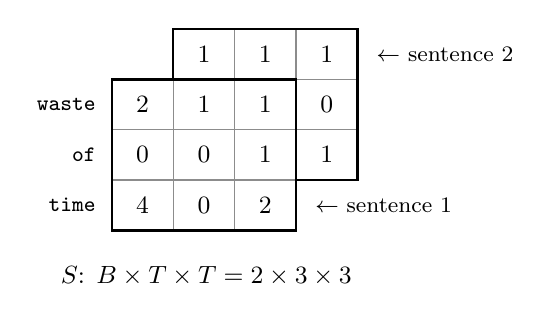
\begin{tikzpicture}
\fill[white] (0.780,0.640) rectangle (3.120,-1.279);
\draw[black!45, fill=white] (0.780,0.640) rectangle (1.560,0.000);
\node[font=\small, text=black] at (1.170,0.320) {$1$};
\draw[black!45, fill=white] (1.560,0.640) rectangle (2.340,0.000);
\node[font=\small, text=black] at (1.950,0.320) {$1$};
\draw[black!45, fill=white] (2.340,0.640) rectangle (3.120,0.000);
\node[font=\small, text=black] at (2.730,0.320) {$1$};
\draw[black!45, fill=white] (0.780,0.000) rectangle (1.560,-0.640);
\node[font=\small, text=black] at (1.170,-0.320) {$1$};
\draw[black!45, fill=white] (1.560,0.000) rectangle (2.340,-0.640);
\node[font=\small, text=black] at (1.950,-0.320) {$0$};
\draw[black!45, fill=white] (2.340,0.000) rectangle (3.120,-0.640);
\node[font=\small, text=black] at (2.730,-0.320) {$0$};
\draw[black!45, fill=white] (0.780,-0.640) rectangle (1.560,-1.279);
\node[font=\small, text=black] at (1.170,-0.959) {$0$};
\draw[black!45, fill=white] (1.560,-0.640) rectangle (2.340,-1.279);
\node[font=\small, text=black] at (1.950,-0.959) {$1$};
\draw[black!45, fill=white] (2.340,-0.640) rectangle (3.120,-1.279);
\node[font=\small, text=black] at (2.730,-0.959) {$1$};
\draw[line width=0.9pt] (0.780,0.640) rectangle (3.120,-1.279);
\node[anchor=west, font=\footnotesize] at (3.240,0.320) {$\leftarrow$ sentence 2};
\fill[white] (0.000,0.000) rectangle (2.340,-1.919);
\draw[black!45, fill=white] (0.000,0.000) rectangle (0.780,-0.640);
\node[font=\small, text=black] at (0.390,-0.320) {$2$};
\draw[black!45, fill=white] (0.780,0.000) rectangle (1.560,-0.640);
\node[font=\small, text=black] at (1.170,-0.320) {$1$};
\draw[black!45, fill=white] (1.560,0.000) rectangle (2.340,-0.640);
\node[font=\small, text=black] at (1.950,-0.320) {$1$};
\draw[black!45, fill=white] (0.000,-0.640) rectangle (0.780,-1.279);
\node[font=\small, text=black] at (0.390,-0.959) {$0$};
\draw[black!45, fill=white] (0.780,-0.640) rectangle (1.560,-1.279);
\node[font=\small, text=black] at (1.170,-0.959) {$0$};
\draw[black!45, fill=white] (1.560,-0.640) rectangle (2.340,-1.279);
\node[font=\small, text=black] at (1.950,-0.959) {$1$};
\draw[black!45, fill=white] (0.000,-1.279) rectangle (0.780,-1.919);
\node[font=\small, text=black] at (0.390,-1.599) {$4$};
\draw[black!45, fill=white] (0.780,-1.279) rectangle (1.560,-1.919);
\node[font=\small, text=black] at (1.170,-1.599) {$0$};
\draw[black!45, fill=white] (1.560,-1.279) rectangle (2.340,-1.919);
\node[font=\small, text=black] at (1.950,-1.599) {$2$};
\draw[line width=0.9pt] (0.000,0.000) rectangle (2.340,-1.919);
\node[anchor=east, font=\footnotesize\ttfamily] at (-0.080,-0.320) {waste};
\node[anchor=east, font=\footnotesize\ttfamily] at (-0.080,-0.959) {of};
\node[anchor=east, font=\footnotesize\ttfamily] at (-0.080,-1.599) {time};
\node[anchor=west, font=\footnotesize] at (2.460,-1.599) {$\leftarrow$ sentence 1};
\node[anchor=north, font=\small] at (1.2,-2.25) {$S$: $B\times T\times T = 2\times3\times3$};
\end{tikzpicture}
\\[14pt]
% AUTO-GENERATED by code/figlib.py helpers -- do not edit
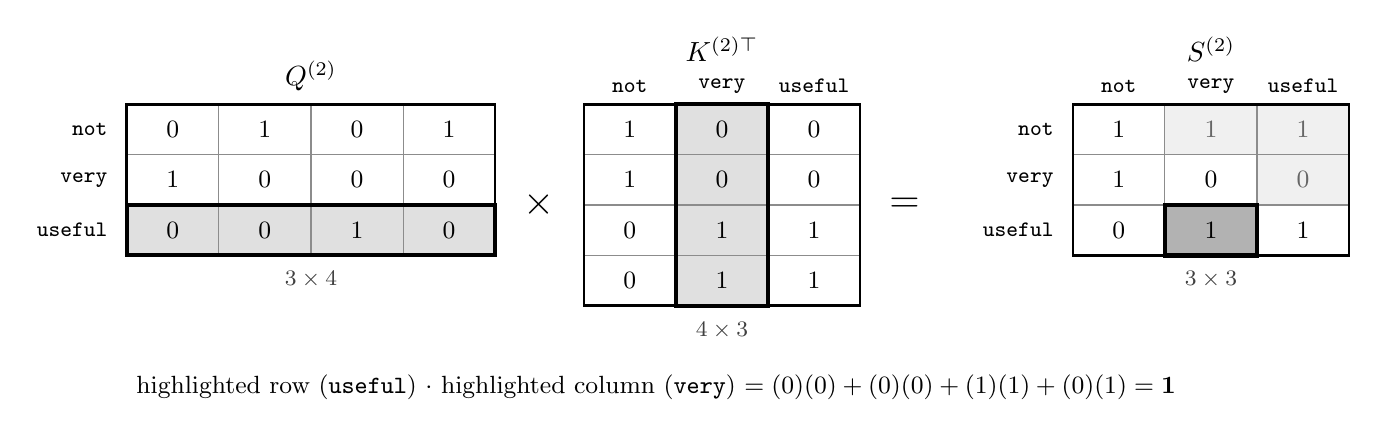
\begin{tikzpicture}[x=1.5cm]
\draw[black!45, fill=white] (0.000,0.000) rectangle (0.780,-0.640);
\node[font=\small, text=black] at (0.390,-0.320) {$0$};
\draw[black!45, fill=white] (0.780,0.000) rectangle (1.560,-0.640);
\node[font=\small, text=black] at (1.170,-0.320) {$1$};
\draw[black!45, fill=white] (1.560,0.000) rectangle (2.340,-0.640);
\node[font=\small, text=black] at (1.950,-0.320) {$0$};
\draw[black!45, fill=white] (2.340,0.000) rectangle (3.120,-0.640);
\node[font=\small, text=black] at (2.730,-0.320) {$1$};
\draw[black!45, fill=white] (0.000,-0.640) rectangle (0.780,-1.279);
\node[font=\small, text=black] at (0.390,-0.959) {$1$};
\draw[black!45, fill=white] (0.780,-0.640) rectangle (1.560,-1.279);
\node[font=\small, text=black] at (1.170,-0.959) {$0$};
\draw[black!45, fill=white] (1.560,-0.640) rectangle (2.340,-1.279);
\node[font=\small, text=black] at (1.950,-0.959) {$0$};
\draw[black!45, fill=white] (2.340,-0.640) rectangle (3.120,-1.279);
\node[font=\small, text=black] at (2.730,-0.959) {$0$};
\draw[black!45, fill=black!12] (0.000,-1.279) rectangle (0.780,-1.919);
\node[font=\small, text=black] at (0.390,-1.599) {$0$};
\draw[black!45, fill=black!12] (0.780,-1.279) rectangle (1.560,-1.919);
\node[font=\small, text=black] at (1.170,-1.599) {$0$};
\draw[black!45, fill=black!12] (1.560,-1.279) rectangle (2.340,-1.919);
\node[font=\small, text=black] at (1.950,-1.599) {$1$};
\draw[black!45, fill=black!12] (2.340,-1.279) rectangle (3.120,-1.919);
\node[font=\small, text=black] at (2.730,-1.599) {$0$};
\draw[line width=1.4pt] (0.000,-1.279) rectangle (3.120,-1.919);
\draw[line width=0.9pt] (0.000,0.000) rectangle (3.120,-1.919);
\node[anchor=east, font=\footnotesize\ttfamily] at (-0.080,-0.320) {not};
\node[anchor=east, font=\footnotesize\ttfamily] at (-0.080,-0.959) {very};
\node[anchor=east, font=\footnotesize\ttfamily] at (-0.080,-1.599) {useful};
\node[anchor=south, font=\normalsize] at (1.560,0.050) {$Q^{(2)}$};
\node[anchor=north, font=\footnotesize, text=black!75] at (1.560,-1.999) {$3\times4$};
\draw[black!45, fill=white] (3.870,0.000) rectangle (4.650,-0.640);
\node[font=\small, text=black] at (4.260,-0.320) {$1$};
\draw[black!45, fill=black!12] (4.650,0.000) rectangle (5.430,-0.640);
\node[font=\small, text=black] at (5.040,-0.320) {$0$};
\draw[black!45, fill=white] (5.430,0.000) rectangle (6.210,-0.640);
\node[font=\small, text=black] at (5.820,-0.320) {$0$};
\draw[black!45, fill=white] (3.870,-0.640) rectangle (4.650,-1.279);
\node[font=\small, text=black] at (4.260,-0.959) {$1$};
\draw[black!45, fill=black!12] (4.650,-0.640) rectangle (5.430,-1.279);
\node[font=\small, text=black] at (5.040,-0.959) {$0$};
\draw[black!45, fill=white] (5.430,-0.640) rectangle (6.210,-1.279);
\node[font=\small, text=black] at (5.820,-0.959) {$0$};
\draw[black!45, fill=white] (3.870,-1.279) rectangle (4.650,-1.919);
\node[font=\small, text=black] at (4.260,-1.599) {$0$};
\draw[black!45, fill=black!12] (4.650,-1.279) rectangle (5.430,-1.919);
\node[font=\small, text=black] at (5.040,-1.599) {$1$};
\draw[black!45, fill=white] (5.430,-1.279) rectangle (6.210,-1.919);
\node[font=\small, text=black] at (5.820,-1.599) {$1$};
\draw[black!45, fill=white] (3.870,-1.919) rectangle (4.650,-2.558);
\node[font=\small, text=black] at (4.260,-2.239) {$0$};
\draw[black!45, fill=black!12] (4.650,-1.919) rectangle (5.430,-2.558);
\node[font=\small, text=black] at (5.040,-2.239) {$1$};
\draw[black!45, fill=white] (5.430,-1.919) rectangle (6.210,-2.558);
\node[font=\small, text=black] at (5.820,-2.239) {$1$};
\draw[line width=1.4pt] (4.650,0.000) rectangle (5.430,-2.558);
\draw[line width=0.9pt] (3.870,0.000) rectangle (6.210,-2.558);
\node[anchor=south, font=\footnotesize\ttfamily] at (4.260,0.020) {not};
\node[anchor=south, font=\footnotesize\ttfamily] at (5.040,0.020) {very};
\node[anchor=south, font=\footnotesize\ttfamily] at (5.820,0.020) {useful};
\node[anchor=south, font=\normalsize] at (5.040,0.420) {$K^{(2)\top}$};
\node[anchor=north, font=\footnotesize, text=black!75] at (5.040,-2.638) {$4\times3$};
\draw[black!45, fill=white] (8.010,0.000) rectangle (8.790,-0.640);
\node[font=\small, text=black] at (8.400,-0.320) {$1$};
\draw[black!45, fill=black!6] (8.790,0.000) rectangle (9.570,-0.640);
\node[font=\small, text=black!60] at (9.180,-0.320) {$1$};
\draw[black!45, fill=black!6] (9.570,0.000) rectangle (10.350,-0.640);
\node[font=\small, text=black!60] at (9.960,-0.320) {$1$};
\draw[black!45, fill=white] (8.010,-0.640) rectangle (8.790,-1.279);
\node[font=\small, text=black] at (8.400,-0.959) {$1$};
\draw[black!45, fill=white] (8.790,-0.640) rectangle (9.570,-1.279);
\node[font=\small, text=black] at (9.180,-0.959) {$0$};
\draw[black!45, fill=black!6] (9.570,-0.640) rectangle (10.350,-1.279);
\node[font=\small, text=black!60] at (9.960,-0.959) {$0$};
\draw[black!45, fill=white] (8.010,-1.279) rectangle (8.790,-1.919);
\node[font=\small, text=black] at (8.400,-1.599) {$0$};
\draw[black!45, fill=black!30] (8.790,-1.279) rectangle (9.570,-1.919);
\node[font=\small, text=black] at (9.180,-1.599) {$1$};
\draw[black!45, fill=white] (9.570,-1.279) rectangle (10.350,-1.919);
\node[font=\small, text=black] at (9.960,-1.599) {$1$};
\draw[line width=1.6pt] (8.790,-1.279) rectangle (9.570,-1.919);
\draw[line width=0.9pt] (8.010,0.000) rectangle (10.350,-1.919);
\node[anchor=east, font=\footnotesize\ttfamily] at (7.930,-0.320) {not};
\node[anchor=east, font=\footnotesize\ttfamily] at (7.930,-0.959) {very};
\node[anchor=east, font=\footnotesize\ttfamily] at (7.930,-1.599) {useful};
\node[anchor=south, font=\footnotesize\ttfamily] at (8.400,0.020) {not};
\node[anchor=south, font=\footnotesize\ttfamily] at (9.180,0.020) {very};
\node[anchor=south, font=\footnotesize\ttfamily] at (9.960,0.020) {useful};
\node[anchor=south, font=\normalsize] at (9.180,0.420) {$S^{(2)}$};
\node[anchor=north, font=\footnotesize, text=black!75] at (9.180,-1.999) {$3\times3$};
\node[font=\Large] at (3.495,-1.279) {$\times$};
\node[font=\Large] at (6.585,-1.279) {$=$};
\node[anchor=north west, font=\small, align=left] at (0,-3.308) {highlighted row (\texttt{useful}) $\cdot$ highlighted column (\texttt{very}) $= (0)(0) + (0)(0) + (1)(1) + (0)(1) = \mathbf{1}$};
\end{tikzpicture}
\\[10pt]
% AUTO-GENERATED by code/figlib.py helpers -- do not edit
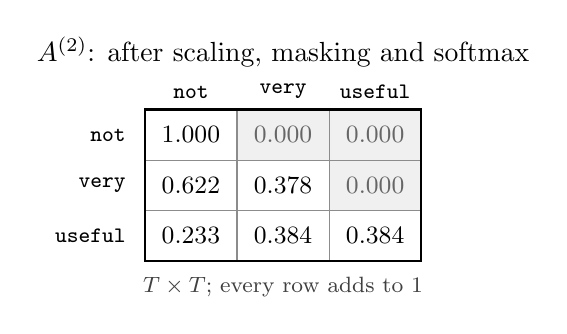
\begin{tikzpicture}[x=1.5cm]
\draw[black!45, fill=white] (0.000,0.000) rectangle (0.780,-0.640);
\node[font=\small, text=black] at (0.390,-0.320) {$1.000$};
\draw[black!45, fill=black!6] (0.780,0.000) rectangle (1.560,-0.640);
\node[font=\small, text=black!60] at (1.170,-0.320) {$0.000$};
\draw[black!45, fill=black!6] (1.560,0.000) rectangle (2.340,-0.640);
\node[font=\small, text=black!60] at (1.950,-0.320) {$0.000$};
\draw[black!45, fill=white] (0.000,-0.640) rectangle (0.780,-1.279);
\node[font=\small, text=black] at (0.390,-0.959) {$0.622$};
\draw[black!45, fill=white] (0.780,-0.640) rectangle (1.560,-1.279);
\node[font=\small, text=black] at (1.170,-0.959) {$0.378$};
\draw[black!45, fill=black!6] (1.560,-0.640) rectangle (2.340,-1.279);
\node[font=\small, text=black!60] at (1.950,-0.959) {$0.000$};
\draw[black!45, fill=white] (0.000,-1.279) rectangle (0.780,-1.919);
\node[font=\small, text=black] at (0.390,-1.599) {$0.233$};
\draw[black!45, fill=white] (0.780,-1.279) rectangle (1.560,-1.919);
\node[font=\small, text=black] at (1.170,-1.599) {$0.384$};
\draw[black!45, fill=white] (1.560,-1.279) rectangle (2.340,-1.919);
\node[font=\small, text=black] at (1.950,-1.599) {$0.384$};
\draw[line width=0.9pt] (0.000,0.000) rectangle (2.340,-1.919);
\node[anchor=east, font=\footnotesize\ttfamily] at (-0.080,-0.320) {not};
\node[anchor=east, font=\footnotesize\ttfamily] at (-0.080,-0.959) {very};
\node[anchor=east, font=\footnotesize\ttfamily] at (-0.080,-1.599) {useful};
\node[anchor=south, font=\footnotesize\ttfamily] at (0.390,0.020) {not};
\node[anchor=south, font=\footnotesize\ttfamily] at (1.170,0.020) {very};
\node[anchor=south, font=\footnotesize\ttfamily] at (1.950,0.020) {useful};
\node[anchor=south, font=\normalsize] at (1.170,0.420) {$A^{(2)}$: after scaling, masking and softmax};
\node[anchor=north, font=\footnotesize, text=black!75] at (1.170,-1.999) {$T\times T$; every row adds to 1};
\end{tikzpicture}

\caption{Top: a batch of $B=2$ sentences. Each sentence keeps its own $3\times4$ matrix $X$ and gets its own
$3\times3$ table $S$. Bottom: the second sentence's table, built by the same multiplication as in
Figure~\ref{fig:qkv}'s machines, and its shares after scaling, masking and softmax.}
\end{figure}

\Picture Two classrooms run the same handshake tournament in parallel, each with its own table. Nobody shakes hands with
the other classroom.

\begin{breaks}
Two real classrooms would need two organisers. Here one multiplication fills both tables; they are separate only
because the numbers are arranged that way.
\end{breaks}

\Exactly Stack the sentences into one block of numbers of shape $B\times T\times d = 2\times3\times4$. The same
machines $W_Q, W_K, W_V$ apply to every token of every sentence, so $Q, K, V$ have shape $B\times T\times d_k$. The
transpose now flips only the last two axes of $K$, and
\[
S = QK^\top \shape{(B\times T\times d_k)(B\times d_k\times T) = B\times T\times T}
\]
is $B$ tournament tables computed side by side: \nScores\ scores in one operation, with no score ever mixing the two
sentences. After the mask and softmax, $O=AV$ has shape $B\times T\times d_k$, and every one of its $B\times T =
\nPreds$ rows will go on to make a next-word guess. Our script checks that sentence 1 gives exactly the same numbers
in the batch as it gave alone.

\Why This is where Chapter 1's history pays off. The RNN had to walk each sentence word by word. Here a batch of $B$
sentences of $T$ tokens is a handful of large matrix multiplications, and those multiplications are what GPUs are
made of.

\Summary{A batch is $B$ separate attention tables computed in one operation, giving $B\times T$ guesses per pass.}

%---------------------------------------------------------------------
\subsection*{3.10\quad How learning shapes the arrows}

Our toy machines were chosen by hand. In a real model, $W_Q$, $W_K$ and $W_V$ start as random numbers and are learned
from the next-word game. Chapter 8 does the bookkeeping; here is the whole idea as a picture.

Every score is $\lVert\bm{q}\rVert\lVert\bm{k}\rVert\cos\theta$, so there are only two ways to change how much one
token attends to another: \emph{turn} the arrows (change the angle) or \emph{stretch} them (change the length).
Training plays the game millions of times. Each time the model guesses the next word, it checks the answer, and
every weight is nudged a tiny step in the direction that would have made the right word a little more likely:
\begin{itemize}
\item if looking more at \tok{waste} would have helped \tok{time} predict \tok{Sorry}, the query of \tok{time} is
turned a little towards the key of \tok{waste} (and that key a little towards the query);
\item if looking at \tok{of} only added noise, the arrows are turned a little apart;
\item if the right choice was clear, the query is stretched, making the softmax more decisive (\S3.7);
\item and the value arrows are turned towards whatever turned out to be useful to hand over.
\end{itemize}

\begin{figure}[h]
\centering
\begin{tikzpicture}[scale=1.25, font=\footnotesize]
\draw[-{Stealth}, thick] (0,0) -- (3.2,0) node[right] {key of \tok{waste}};
\draw[-{Stealth}, thick, black!65] (0,0) -- (-1.2,1.3) node[left, text=black] {key of \tok{of}};
\draw[-{Stealth}, thick, dashed, black!65] (0,0) -- (0.4,1.5) node[above, text=black] {query of \tok{time}, at the start};
\draw[-{Stealth}, very thick] (0,0) -- (2.7,1.2) node[right] {query after training};
\draw[-{Stealth}, black!60] (0.31,1.16) arc[start angle=75, end angle=30, radius=1.2];
\end{tikzpicture}
\caption{Learning as turning and stretching arrows (schematic, not to scale). The query is turned towards the key
that helped, away from the one that did not, and stretched to be more confident. Training never moves the arrows
directly; it changes the machines $W_Q, W_K, W_V$ that produce them.}
\end{figure}

\begin{breaks}
The figure turns one arrow. Training turns the \emph{machines}, so every arrow those machines produce turns
together, including arrows for sentences that are not in this batch.
\end{breaks}

That last point makes this powerful. A nudge learned from \tok{waste of time} also moves the arrows produced for
\tok{waste of money} and \tok{waste of effort}, because those words have nearby arrows (Requirement 1). That is how
a model trained on finitely many sentences handles sentences it has never seen, the exact thing the counting
notebook of \S1.3 could not do.

\Summary{Learning only turns and stretches arrows, by adjusting the machines that make them, so lessons spread to
similar words.}

%---------------------------------------------------------------------
\subsection*{3.11\quad What we built, and the next failure}

\begin{principle}{attention is a soft lookup table}
A Python dictionary takes a query, finds the one key that matches \emph{exactly}, and returns its value. Attention
does the same, softly: every key matches a little, measured by a dot product, and you get a blend of all the values.
Because ``a little'' is a smooth number, the lookup can be learned. The same pattern appears whenever a system must
pick from candidates by relevance: a search engine ranking documents, a recommender ranking products, or the
retriever in an AI agent's memory system, which scores stored memories against the current conversation and decides
how much of each one reaches the model.
\end{principle}

\Predict Swap the first two tokens and feed \tok{of waste time}. Will the output for \tok{time} change?

The output for \tok{time} is
\[ \bm{o}_{\text{time}} = \oTimeSwap, \]
\emph{identical} to before. The mask decides who may look at whom, but the scores themselves cannot tell \tok{waste
of} from \tok{of waste}: to \tok{time}, its past is a bag, not a sequence. We have quietly lost Requirement 2, the
very thing the RNN gave us for free, and we are back to the bag of words of \S1.4. Chapter 4 fixes it, and the fix
(RoPE) turns out to be a \emph{rotation} of exactly these query and key arrows, by an angle that depends on the
position.

\begin{wrongidea}{3.10}
\emph{Attention already knows the order of the words.} Masking is about order, so it seems order must be handled. But none of $W_Q$, $W_K$, $W_V$
sees a position. The mask only says which tokens are visible; among the visible ones, attention cannot tell who
came first.
\end{wrongidea}

\begin{checkq}
Feed \tok{of waste time} instead of \tok{waste of time}. What happens to the output for \tok{time}?
\begin{options}
\item It is unchanged: \tok{time} sees the same set of earlier tokens, and nothing in the scores knows their order.
\item It changes, because the causal mask encodes word order.
\item It changes, because \tok{waste}'s value is now in a different row.
\item It changes, because the scores are percentages of position.
\end{options}
\end{checkq}

\Summary{Attention is a learnable soft lookup that meets Requirements 3 and 4, but on its own it cannot tell word
order.}

%---------------------------------------------------------------------
\begin{lookingback}
(1) Chapter 1: why does one sentence of $T$ tokens give $T$ training exercises? (2) Chapter 1: which requirement did
the RNN fail that attention now meets, and which one did attention lose? (3) Chapter 2: where do the rows of $X$ come
from? (4) Chapter 2: why does a tokenizer split a rare word into pieces instead of giving it its own token?
\end{lookingback}

\subsection*{Exercises}

\begin{exercise}
Compute by hand the attention output for the token \tok{of}. Then explain, using only the geometry of
$\bm{q}_{\text{of}}$ and the keys, why its two shares are equal.
\end{exercise}

\begin{exercise}
A model has $d_k=256$. Without scaling, roughly how far apart would the scores of unrelated tokens typically be? What
would you divide by, and why that number?
\end{exercise}

\begin{exercise}
Fill the gaps for the token \tok{useful} in the second sentence of \S3.9. Its raw scores are $(0, 1, 1)$. After
dividing by $\sqrt{d_k}$ they are $(\rule{1em}{0.4pt}, \rule{1em}{0.4pt}, \rule{1em}{0.4pt})$. Exponentiate, divide by the
total, and check your answer against the last row of $A^{(2)}$.
\end{exercise}

\begin{exercise}
A second customer has clues $\nThreeClTwo$ with the same importances $\nThreeW$. Compute the churn score. Is the
customer arrow pointing with or against the importance arrow?
\end{exercise}

\subsection*{Answers to Chapter 3}
\small
\textbf{Check yourself 3.1.} (b). (a) is M3.1: the arrow does not change with context. (c) is the uniform average
that \S3.1 showed cannot learn. (d) is a real issue (Chapter 4), but even with positions, one arrow cannot see its
neighbours.

\textbf{Check yourself 3.2.} (b). (a) is M3.8: $\bm{b}$ wins on dot product only because it is longer. (c) mixes up
``positive'' with ``equal''. (d): the angles answer it without drawing.

\textbf{Check yourself 3.3.} (a). (b) and (c) are M3.9: the transpose changes no arrow. (d) is wrong because $QK$ is
not defined.

\textbf{Check yourself 3.4.} (b). (a) is M3.4, (c) is M3.6, (d) is M3.5.

\textbf{Check yourself 3.5.} (b). (a) is M3.7: the mask is also what lets all rows train together. (c) is M3.2.
(d) is false: \tok{time} gives \apctTime\% to itself.

\textbf{Check yourself 3.6.} (a), for reason (i). Softmax gives $(\nThreeSoft)$ for both lists. (b) is M3.2. (c) is
M3.11: dividing by the total would give $(\nThreeRatioB)$, the shift option (c) expects. (d) is M3.8.

\textbf{Check yourself 3.7.} (b). (a) is M3.3. (c) is M3.2: softmax does that. (d) is true in the toy only.

\textbf{Check yourself 3.8.} (a). (b) is M3.10. (c): the rows moved, but the set of value arrows \tok{time} blends is
the same. (d) mixes two wrong ideas.

\textbf{Looking back.} (1) Each prefix asks for its own next word, and the mask lets all prefixes be answered in one
pass. (2) Attention meets Requirement 3 (direct reach) and loses Requirement 2 (order). (3) Each token id picks one
row of the embedding table. (4) So the vocabulary stays a fixed size and no word is ever unknown: a rare word becomes
known pieces.

\textbf{Exercise 3.1.} $\bm{q}_{\text{of}}=(0,1,0,0)$ points along the second direction only. Both
$\bm{k}_{\text{waste}}$ and $\bm{k}_{\text{of}}$ have 0 there: both are at right angles to the query, so both scores
are 0, the softmax of $(0,0)$ is $(0.5,0.5)$, and $\bm{o}_{\text{of}} = 0.5\,\bm{v}_{\text{waste}}+0.5\,\bm{v}_{\text{of}}
= \oOf$. A query at right angles to every key has nothing to prefer, and attention falls back to the plain average of
\S3.1. \emph{Uniform attention is what ``no information'' looks like.}

\textbf{Exercise 3.2.} About $\sqrt{256}=\nThreeRootTwoFiftySix$ points, enough for softmax to put nearly all its
weight on one key at random. Divide by $\sqrt{256}$ to bring the typical spread back to about one point, whatever
$d_k$ is.

\textbf{Exercise 3.3.} $(0, 0.5, 0.5)$; the two equal scores give equal shares, and the last row of $A^{(2)}$ shows the
result. The strategy that works: do one row at a time, and check the shares add to 1.

\textbf{Exercise 3.4.} $\nThreeClTwo\cdot\nThreeW = \nThreeScoreTwo$. Negative: the customer arrow points partly
against the importance arrow.
\normalsize

\subsection*{What you now know}
\begin{itemize}
\item The dot product as weighted clues, as a shadow, and as lengths times agreement, and why the two formulas match.
\item A matrix as recipe cards and as a machine that moves arrows; the transpose as standing keys up as columns.
\item Queries, keys and values, and a full attention computation by hand, with masking and softmax.
\item Why softmax uses $e^x$, why scores are divided by $\sqrt{d_k}$, and how a batch runs in one operation.
\item Learning as turning and stretching arrows, and the next failure: attention alone ignores order.
\end{itemize}
